%!TEX root = ../ICR.tex
\chapter{Resultados y Evaluación Comparativa \label{cap:AnalisisDeResultados}}

Este capítulo presenta el análisis integral de los resultados obtenidos mediante la metodología unificada desarrollada para la detección de noticias falsas en español. Los resultados se organizan siguiendo la estructura evolutiva de la metodología: comenzando con la validación del flujo de datos de datos común, continuando con la evaluación de los modelos clásicos optimizados con algoritmos metaheurísticos (que establecen la línea base), progresando hacia los resultados del modelo Transformer DistilBERT, y culminando con una evaluación comparativa integral que justifica la selección del modelo final.

El análisis estadístico se fundamenta en un marco de evaluación unificado que emplea las métricas definidas en la metodología: Exactitud (Accuracy), Precisión (Precision), Exhaustividad (Recall), F1-Score y Especificidad. \textbf{Criterio fundamental:} Todos los experimentos se ejecutaron bajo condiciones experimentales idénticas para garantizar comparabilidad objetiva: mismo corpus, misma división de datos (70\% entrenamiento, 10\% validación, 20\% prueba), y mismo protocolo de validación.

\section{Validación del Flujo de Datos y Representaciones}
\label{sec:validacion_pipeline_datos}

Antes de proceder con la evaluación de modelos, se validó la robustez del flujo de datos de procesamiento desarrollado, que constituye la base común para ambos enfoques de modelado.

\subsection{Características del Corpus Unificado Final}

El corpus utilizado para todos los experimentos presentaba inicialmente las siguientes características tras el proceso de unificación y limpieza:

\begin{table}[htbp]
\centering
\adjustbox{width=\textwidth,center}{%
\footnotesize
\begin{tabular}{|c|l|l|c|c|l|c|}
\hline
\rowcolor{UAMAzcapo}
\textbf{\textcolor{white}{ID}} & \textbf{\textcolor{white}{Nombre del Corpus}} & \textbf{\textcolor{white}{Autores Principales}} & \textbf{\textcolor{white}{Año}} & \textbf{\textcolor{white}{Noticias}} & \textbf{\textcolor{white}{Características}} & \textbf{\textcolor{white}{Ref.}} \\
\hline
\rowcolor{UAMIztapalapaLight!50}
1 & \begin{tabular}[t]{@{}l@{}}Spanish Fake News Corpus\\(IberLEF)\end{tabular} & \begin{tabular}[t]{@{}l@{}}Posadas-Durán, J.P.\\Gómez-Adorno, H.\end{tabular} & 2019-2021 & 971 & \begin{tabular}[t]{@{}l@{}}Análisis estilométrico\\Múltiples versiones\end{tabular} & \cite{posadas2019detection} \\
\hline
\rowcolor{UAMCuajimalpaLight!50}
2 & \begin{tabular}[t]{@{}l@{}}Conjunto de datos Zules Acosta\\(UPM)\end{tabular} & Acosta, F.A.Z. & 2019 & 598 & \begin{tabular}[t]{@{}l@{}}Trabajo fin de maestría\\Extracción web verificada\end{tabular} & \cite{acosta2019construccion} \\
\hline
\rowcolor{UAMLermaLight!50}
3 & \begin{tabular}[t]{@{}l@{}}Conjunto de datos Tretiakov\\(Kaggle)\end{tabular} & \begin{tabular}[t]{@{}l@{}}Tretiakov, A.\\Martín García, A.\end{tabular} & 2022 & 1,958 & \begin{tabular}[t]{@{}l@{}}Aprendizaje automático\\Disponible públicamente\end{tabular} & \cite{tretiakov2022detection} \\
\hline
\rowcolor{UAMXochimilcoLight!50}
4 & \begin{tabular}[t]{@{}l@{}}Spanish Political Fake News\\Conjunto de datos\end{tabular} & \begin{tabular}[t]{@{}l@{}}Blanco-Fernández, Y.\\Otero-Vizoso, J.\end{tabular} & 2024 & 57,231 & \begin{tabular}[t]{@{}l@{}}Temática política\\Modelos BERT/RoBERTa\end{tabular} & \cite{blanco2024enhancing} \\
\hline
\rowcolor{UAMAzcapo}
\multicolumn{5}{|c|}{\textbf{\textcolor{white}{TOTAL CORPUS ACADÉMICOS}}} & \textbf{\textcolor{white}{60,758}} & \textbf{\textcolor{white}{Cuatro fuentes}} \\
\hline
\end{tabular}
}
\caption{Corpus académicos utilizados para la construcción del conjunto de datos unificado.}
\label{tab:corpus_academicos_resultados}
\end{table}

\subsubsection{Configuración de Representación Textual}

Como se detalló en capitulos anteriores, la representación textual se basó en TF-IDF con la siguiente configuración específica para los experimentos:

\begin{itemize}
    \item \textbf{Vocabulario inicial:} 5,000 términos más frecuentes del corpus
    \item \textbf{Reducción de dimensionalidad:} Selección del 10\% más discriminativo (500 características)
    \item \textbf{Criterio de selección:} Test chi-cuadrado para identificar características más relevantes
    \item \textbf{Representación final:} Matriz dispersa de 500 dimensiones por documento
    \item \textbf{Trade-off (compensación) identificado:} La selección de más características tiende a mejorar las métricas de clasificación pero deteriora significativamente el rendimiento computacional de los algoritmos metaheurísticos
\end{itemize}

\textbf{Justificación de la configuración:} La selección de 500 características (10\% del vocabulario) representa un balance óptimo entre capacidad discriminativa y eficiencia computacional. Experimentos preliminares con más de 1,000 características mostraron mejoras marginales en exactitud (<2\%) a costa de incrementos importantes en tiempo de convergencia (>300\%), haciendo inviable la optimización metaheurística en tiempos razonables.

\subsubsection{Arquitectura del Clasificador}

Todos los algoritmos metaheurísticos, detallados en capitulos anteriores, optimizaron un clasificador logístico binario con las siguientes características:

\begin{itemize}
    \item \textbf{Función de activación:} Sigmoide para clasificación binaria
    \item \textbf{Parámetros optimizados:} Selección de características, pesos del modelo y umbrales de decisión
    \item \textbf{Función objetivo:} Maximización de la exactitud en el conjunto de entrenamiento
\end{itemize}

\subsection{Implementación y Configuración de Algoritmos Metaheurísticos}
\label{subsec:implementacion_algoritmos}

La tabla \ref{tab:configuracion_algoritmos_metaheuristicos} (ver tabla \ref{tab:configuracion_algoritmos_metaheuristicos}) presenta la configuración detallada de parámetros para cada algoritmo metaheurístico implementado. Estos valores fueron establecidos siguiendo las mejores prácticas reportadas en la literatura y ajustados experimentalmente para el dominio específico de detección de noticias falsas.

\begin{table}[htbp]
\centering
\adjustbox{width=\textwidth,center}{%
\footnotesize
\begin{tabular}{|l|l|l|l|l|l|}
\hline
\rowcolor{UAMAzcapo}
\textbf{\textcolor{white}{Parámetro}} & \textbf{\textcolor{white}{MSA}} & \textbf{\textcolor{white}{SS}} & \textbf{\textcolor{white}{GA}} & \textbf{\textcolor{white}{VNS}} & \textbf{\textcolor{white}{PSO}} \\
\hline
\rowcolor{UAMIztapalapaLight!50}
\textbf{Iteraciones/Generaciones} & 31 temperaturas & 10 iteraciones & 20 generaciones & 20 iteraciones & 20 iteraciones \\
\hline
\rowcolor{UAMCuajimalpaLight!50}
\textbf{Población/Agentes} & 5 multiarranques & 50 soluciones & 50 individuos & 1 solución & 30 partículas \\
\hline
\rowcolor{UAMLermaLight!50}
\textbf{Parámetro Principal 1} & \begin{tabular}[t]{@{}l@{}}Temp. inicial:\\1000\end{tabular} & \begin{tabular}[t]{@{}l@{}}RefSet:\\5 soluciones\end{tabular} & \begin{tabular}[t]{@{}l@{}}Tasa mutación:\\0.1\end{tabular} & \begin{tabular}[t]{@{}l@{}}k\_max:\\5 vecindarios\end{tabular} & \begin{tabular}[t]{@{}l@{}}Factor inercia:\\0.5\end{tabular} \\
\hline
\rowcolor{UAMXochimilcoLight!50}
\textbf{Parámetro Principal 2} & \begin{tabular}[t]{@{}l@{}}Temp. final:\\1.24\end{tabular} & \begin{tabular}[t]{@{}l@{}}Combinaciones:\\10 por iteración\end{tabular} & \begin{tabular}[t]{@{}l@{}}Torneo:\\3 competidores\end{tabular} & \begin{tabular}[t]{@{}l@{}}Estrategia:\\k elementos\end{tabular} & \begin{tabular}[t]{@{}l@{}}Coef. cognitivo:\\1.5\end{tabular} \\
\hline
\rowcolor{UAMAzcapoLight!50}
\textbf{Parámetro Principal 3} & \begin{tabular}[t]{@{}l@{}}Factor enfriamiento:\\0.8\end{tabular} & \begin{tabular}[t]{@{}l@{}}Mejora:\\Mutación aleatoria\end{tabular} & \begin{tabular}[t]{@{}l@{}}Cruce:\\Un punto\end{tabular} & \begin{tabular}[t]{@{}l@{}}Aceptación:\\Solo mejora\end{tabular} & \begin{tabular}[t]{@{}l@{}}Coef. social:\\1.5\end{tabular} \\
\hline
\rowcolor{UAMIztapalapaLight!50}
\textbf{Característica Especial} & \begin{tabular}[t]{@{}l@{}}100 pasos por\\temperatura\end{tabular} & \begin{tabular}[t]{@{}l@{}}Combinación\\sistemática\end{tabular} & \begin{tabular}[t]{@{}l@{}}Selección\\determinística\end{tabular} & \begin{tabular}[t]{@{}l@{}}Reinicio a k=1\\tras mejora\end{tabular} & \begin{tabular}[t]{@{}l@{}}Velocidad\\gaussiana inicial\end{tabular} \\
\hline
\rowcolor{UAMCuajimalpaLight!50}
\textbf{Filosofía de Búsqueda} & \begin{tabular}[t]{@{}l@{}}Aceptación\\probabilística\end{tabular} & \begin{tabular}[t]{@{}l@{}}Combinación\\estructurada\end{tabular} & \begin{tabular}[t]{@{}l@{}}Evolución\\darwiniana\end{tabular} & \begin{tabular}[t]{@{}l@{}}Cambio de\\vecindarios\end{tabular} & \begin{tabular}[t]{@{}l@{}}Inteligencia\\de enjambre\end{tabular} \\
\hline
\end{tabular}
}
\caption{Configuración detallada de parámetros para los cinco algoritmos metaheurísticos implementados.}
\label{tab:configuracion_algoritmos_metaheuristicos}
\end{table}

\subsubsection{Justificación de Parámetros Seleccionados}

Los parámetros establecidos se fundamentan en:

\begin{itemize}
    \item \textbf{Literatura especializada:} Valores base extraídos de trabajos originales para cada algoritmo
    \item \textbf{Balance exploración-explotación:} Configuración para evitar convergencia prematura
    \item \textbf{Eficiencia computacional:} Límites de iteraciones para tiempos de ejecución razonables
    \item \textbf{Estabilidad estadística:} Parámetros que garantizan reproducibilidad de resultados
\end{itemize}

\subsection{Pseudocódigos de los Algoritmos Implementados}
\label{subsec:pseudocodigos_algoritmos}

\subsubsection{Función de Evaluación Común}

Todos los algoritmos metaheurísticos utilizan una función de evaluación unificada que implementa un clasificador logístico binario para garantizar comparabilidad directa entre enfoques. A continuación se presenta el pseudocódigo detallado de la función implementada (ver tabla \ref{tab:funcion_evaluacion}):

\begin{table}[htbp]
\centering
\adjustbox{width=\textwidth,center}{%
\scriptsize
\begin{tabular}{|l|l|}
\hline
\rowcolor{UAMAzcapo}
\multicolumn{2}{|l|}{\textbf{\textcolor{white}{Función: evaluar\_solucion}$(solucion, pesos, umbrales, X, y)$}} \\
\hline
\textbf{Entrada:} & Índices de características, pesos, umbrales, datos $X$, etiquetas $y$ \\
\hline
\textbf{Salida:} & Tupla (exactitud, predicciones) \\
\hline
\rowcolor{UAMAzcapoLight!40}
\multicolumn{2}{|l|}{\textbf{Proceso de clasificación logística:}} \\
\hline
\multicolumn{2}{|l|}{Para cada instancia $i$ en $X$:} \\
\multicolumn{2}{|l|}{\quad $caracteristicas\_activas \leftarrow X[i, solucion]$} \\
\multicolumn{2}{|l|}{\quad $x\_binario \leftarrow (caracteristicas\_activas \geq umbrales)$.astype(int)} \\
\multicolumn{2}{|l|}{\quad $logit \leftarrow$ np.dot($pesos$, $x\_binario$)} \\
\multicolumn{2}{|l|}{\quad $probabilidad \leftarrow \frac{1}{1 + \exp(-logit)}$} \\
\multicolumn{2}{|l|}{\quad $clase\_predicha \leftarrow 1$ si $probabilidad \geq 0.5$, $0$ en otro caso} \\
\multicolumn{2}{|l|}{$exactitud \leftarrow$ accuracy\_score($y$, $predicciones$)} \\
\multicolumn{2}{|l|}{\textbf{Retornar} ($exactitud$, np.array($predicciones$))} \\
\hline
\end{tabular}
}
\caption{Función de evaluación común utilizada por todos los algoritmos metaheurísticos.}
\label{tab:funcion_evaluacion}
\end{table}

\newpage

\subsubsection{Multi-Start Simulated Annealing (MSA)}

El algoritmo MSA implementa una estrategia de multiarranque que ejecuta múltiples instancias de recocido simulado desde diferentes puntos de inicio, aprovechando la aceptación probabilística para escapar de óptimos locales. En la tabla \ref{tab:pseudocodigo_msa} (ver tabla \ref{tab:pseudocodigo_msa}) se presenta el pseudocódigo detallado del algoritmo implementado.

\begin{table}[htbp]
\centering
\adjustbox{width=\textwidth,center}{%
\scriptsize
\begin{tabular}{|l|l|}
\hline
\rowcolor{UAMAzcapo}
\multicolumn{2}{|l|}{\textbf{\textcolor{white}{Algoritmo MSA - Multi-Start Simulated Annealing}}} \\
\hline
\textbf{Entrada:} & $TI=1000$, $TF=1$, $\alpha=0.8$, $pasos=100$, $puntos=5$ \\
\hline
\textbf{Salida:} & Mejor solución $(sol^*, pesos^*, umbrales^*)$ \\
\hline
\rowcolor{UAMAzcapoLight!40}
\multicolumn{2}{|l|}{\textbf{0. Carga y preprocesamiento de datos:}} \\
\hline
\multicolumn{2}{|l|}{Cargar corpus TF-IDF desde archivo CSV} \\
\multicolumn{2}{|l|}{Dividir datos: 80\% entrenamiento, 10\% validación, 10\% pruebas} \\
\multicolumn{2}{|l|}{Aplicar SelectPercentile(percentile=10) para reducir características} \\
\hline
\rowcolor{UAMAzcapoLight!40}
\multicolumn{2}{|l|}{\textbf{1. Inicialización multiarranque:}} \\
\hline
\multicolumn{2}{|l|}{Para $k = 1$ hasta $puntos=5$:} \\
\multicolumn{2}{|l|}{\quad $soluciones[k] \leftarrow$ np.random.randint(0, num\_caracteristicas, size=num\_caracteristicas)} \\
\multicolumn{2}{|l|}{\quad $pesos[k] \leftarrow$ np.random.uniform(-10, 10, size=num\_caracteristicas)} \\
\multicolumn{2}{|l|}{\quad $umbrales[k] \leftarrow$ np.random.uniform(0, 1, size=num\_caracteristicas)} \\
\multicolumn{2}{|l|}{\quad $evaluaciones[k] \leftarrow$ evaluar\_solucion$(soluciones[k], pesos[k], umbrales[k])$} \\
\hline
\rowcolor{UAMAzcapoLight!40}
\multicolumn{2}{|l|}{\textbf{2. Proceso de enfriamiento gradual:}} \\
\hline
\multicolumn{2}{|l|}{$TA \leftarrow TI = 1000$} \\
\multicolumn{2}{|l|}{\textbf{Mientras} $TA > TF = 1$:} \\
\multicolumn{2}{|l|}{\quad Para $k = 1$ hasta $puntos$:} \\
\multicolumn{2}{|l|}{\quad \quad Para $paso = 1$ hasta $pasos=100$:} \\
\multicolumn{2}{|l|}{\quad \quad \quad Generar solución vecina modificando elemento aleatorio} \\
\multicolumn{2}{|l|}{\quad \quad \quad $\Delta E \leftarrow eval\_vecina - evaluaciones[k]$} \\
\multicolumn{2}{|l|}{\quad \quad \quad \textbf{Si} $\Delta E > 0$ \textbf{o} random() $< \exp(\Delta E / TA)$:} \\
\multicolumn{2}{|l|}{\quad \quad \quad \quad Aceptar solución vecina} \\
\multicolumn{2}{|l|}{\quad $TA \leftarrow TA \times \alpha = TA \times 0.8$} \\
\hline
\rowcolor{UAMAzcapoLight!40}
\multicolumn{2}{|l|}{\textbf{3. Evaluación final:}} \\
\hline
\multicolumn{2}{|l|}{$idx\_mejor \leftarrow \arg\max(evaluaciones)$} \\
\multicolumn{2}{|l|}{Evaluar mejor solución en conjunto de pruebas} \\
\multicolumn{2}{|l|}{Generar reporte de clasificación y matriz de confusión} \\
\multicolumn{2}{|l|}{Guardar gráficas de convergencia y resultados} \\
\hline
\end{tabular}
}
\caption{Pseudocódigo completo del algoritmo Multi-Start Simulated Annealing (MSA).}
\label{tab:pseudocodigo_msa}
\end{table}

\subsubsection{Scatter Search (SS)}

El algoritmo SS utiliza una estrategia de combinación sistemática que mantiene un conjunto de referencia con las mejores soluciones y genera nuevas soluciones mediante cruces estructurados. En la tabla \ref{tab:pseudocodigo_ss} (ver tabla \ref{tab:pseudocodigo_ss}) se presenta el pseudocódigo detallado del algoritmo implementado.

\begin{table}[htbp]
\centering
\adjustbox{width=\textwidth,center}{%
\scriptsize
\begin{tabular}{|l|l|}
\hline
\rowcolor{UAMAzcapo}
\multicolumn{2}{|l|}{\textbf{\textcolor{white}{Algoritmo SS - Scatter Search}}} \\
\hline
\textbf{Entrada:} & $P=50$, $b=5$, $max\_iteraciones=10$, $num\_combinaciones=10$ \\
\hline
\textbf{Salida:} & Mejor solución del RefSet final \\
\hline
\rowcolor{UAMAzcapoLight!40}
\multicolumn{2}{|l|}{\textbf{0. Carga y preprocesamiento de datos:}} \\
\hline
\multicolumn{2}{|l|}{Cargar corpus TF-IDF desde archivo CSV} \\
\multicolumn{2}{|l|}{Dividir datos: 80\% entrenamiento, 10\% validación, 10\% pruebas} \\
\multicolumn{2}{|l|}{Aplicar SelectPercentile(percentile=10) para reducir características} \\
\hline
\rowcolor{UAMAzcapoLight!40}
\multicolumn{2}{|l|}{\textbf{1. Generación de población inicial diversa:}} \\
\hline
\multicolumn{2}{|l|}{Para $i = 1$ hasta $P=50$: generar solución aleatoria y evaluar} \\
\multicolumn{2}{|l|}{Ordenar población por score descendente} \\
\multicolumn{2}{|l|}{$ref\_set \leftarrow poblacion[:b]$ (mejores $b=5$ soluciones)} \\
\hline
\rowcolor{UAMAzcapoLight!40}
\multicolumn{2}{|l|}{\textbf{2. Proceso iterativo de mejora:}} \\
\hline
\multicolumn{2}{|l|}{Para $iteracion = 1$ hasta $max\_iteraciones=10$:} \\
\multicolumn{2}{|l|}{\quad Para $c = 1$ hasta $num\_combinaciones=10$:} \\
\multicolumn{2}{|l|}{\quad \quad Seleccionar aleatoriamente $s1, s2 \in ref\_set$} \\
\multicolumn{2}{|l|}{\quad \quad Aplicar cruce en punto aleatorio + mutación} \\
\multicolumn{2}{|l|}{\quad \quad Evaluar nueva solución} \\
\multicolumn{2}{|l|}{\quad Actualizar $ref\_set$ con mejores $b$ soluciones} \\
\hline
\rowcolor{UAMAzcapoLight!40}
\multicolumn{2}{|l|}{\textbf{3. Evaluación final:}} \\
\hline
\multicolumn{2}{|l|}{Evaluar mejor solución del RefSet en conjunto de pruebas} \\
\multicolumn{2}{|l|}{Generar reporte de clasificación y matriz de confusión} \\
\multicolumn{2}{|l|}{Guardar gráficas de convergencia y resultados} \\
\hline
\end{tabular}
}
\caption{Pseudocódigo completo del algoritmo Scatter Search (SS).}
\label{tab:pseudocodigo_ss}
\end{table}

\subsubsection{Genetic Algorithm (GA)}

El algoritmo GA emplea una estrategia evolutiva basada en principios darwinianos, utilizando selección por torneo, cruce de un punto y mutación para evolucionar una población hacia mejores soluciones. En la tabla \ref{tab:pseudocodigo_ga} (ver tabla \ref{tab:pseudocodigo_ga}) se presenta el pseudocódigo detallado del algoritmo implementado.

\begin{table}[htbp]
\centering
\adjustbox{width=\textwidth,center}{%
\scriptsize
\begin{tabular}{|l|l|}
\hline
\rowcolor{UAMAzcapo}
\multicolumn{2}{|l|}{\textbf{\textcolor{white}{Algoritmo GA - Genetic Algorithm}}} \\
\hline
\textbf{Entrada:} & $num\_generaciones=20$, $tam\_poblacion=50$, $tasa\_mutacion=0.1$, $tam\_torneo=3$ \\
\hline
\textbf{Salida:} & Mejor individuo global encontrado \\
\hline
\rowcolor{UAMAzcapoLight!40}
\multicolumn{2}{|l|}{\textbf{0. Carga y preprocesamiento de datos:}} \\
\hline
\multicolumn{2}{|l|}{Cargar corpus TF-IDF desde archivo CSV} \\
\multicolumn{2}{|l|}{Dividir datos: 80\% entrenamiento, 10\% validación, 10\% pruebas} \\
\multicolumn{2}{|l|}{Aplicar SelectPercentile(percentile=10) para reducir características} \\
\hline
\rowcolor{UAMAzcapoLight!40}
\multicolumn{2}{|l|}{\textbf{1. Inicialización y proceso evolutivo:}} \\
\hline
\multicolumn{2}{|l|}{Generar población inicial de $tam\_poblacion=50$ individuos} \\
\multicolumn{2}{|l|}{Para $gen = 1$ hasta $num\_generaciones=20$:} \\
\multicolumn{2}{|l|}{\quad Evaluar toda la población} \\
\multicolumn{2}{|l|}{\quad Actualizar mejor global si es necesario} \\
\multicolumn{2}{|l|}{\quad Para $i = 1$ hasta $tam\_poblacion // 2$:} \\
\multicolumn{2}{|l|}{\quad \quad Seleccionar padres por torneo (k=3)} \\
\multicolumn{2}{|l|}{\quad \quad Aplicar cruce de un punto} \\
\multicolumn{2}{|l|}{\quad \quad Aplicar mutación con probabilidad 0.1} \\
\hline
\rowcolor{UAMAzcapoLight!40}
\multicolumn{2}{|l|}{\textbf{2. Evaluación final:}} \\
\hline
\multicolumn{2}{|l|}{Evaluar mejor individuo global en conjunto de pruebas} \\
\multicolumn{2}{|l|}{Generar reporte de clasificación y matriz de confusión} \\
\multicolumn{2}{|l|}{Guardar gráficas de convergencia y resultados} \\
\hline
\end{tabular}
}
\caption{Pseudocódigo completo del Algoritmo Genético (GA).}
\label{tab:pseudocodigo_ga}
\end{table}

\subsubsection{Variable Neighborhood Search (VNS)}

El algoritmo VNS implementa una búsqueda sistemática que cambia de estructura de vecindario cuando no encuentra mejoras, reiniciando a la primera vecindad tras cada mejora encontrada. En la tabla \ref{tab:pseudocodigo_vns} (ver tabla \ref{tab:pseudocodigo_vns}) se presenta el pseudocódigo detallado del algoritmo implementado.

\begin{table}[htbp]
\centering
\adjustbox{width=\textwidth,center}{%
\scriptsize
\begin{tabular}{|l|l|}
\hline
\rowcolor{UAMAzcapo}
\multicolumn{2}{|l|}{\textbf{\textcolor{white}{Algoritmo VNS - Variable Neighborhood Search}}} \\
\hline
\textbf{Entrada:} & $max\_iteraciones=20$, $k\_max=5$ \\
\hline
\textbf{Salida:} & Mejor solución global encontrada \\
\hline
\rowcolor{UAMAzcapoLight!40}
\multicolumn{2}{|l|}{\textbf{0. Carga y preprocesamiento de datos:}} \\
\hline
\multicolumn{2}{|l|}{Cargar corpus TF-IDF desde archivo CSV} \\
\multicolumn{2}{|l|}{Dividir datos: 80\% entrenamiento, 10\% validación, 10\% pruebas} \\
\multicolumn{2}{|l|}{Aplicar SelectPercentile(percentile=10) para reducir características} \\
\hline
\rowcolor{UAMAzcapoLight!40}
\multicolumn{2}{|l|}{\textbf{1. Inicialización y búsqueda en vecindades:}} \\
\hline
\multicolumn{2}{|l|}{Generar solución inicial aleatoria} \\
\multicolumn{2}{|l|}{Para $i = 1$ hasta $max\_iteraciones=20$:} \\
\multicolumn{2}{|l|}{\quad $k \leftarrow 1$} \\
\multicolumn{2}{|l|}{\quad \textbf{Mientras} $k \leq k\_max=5$:} \\
\multicolumn{2}{|l|}{\quad \quad Generar vecino modificando $k$ elementos aleatorios} \\
\multicolumn{2}{|l|}{\quad \quad \textbf{Si mejora}: aceptar y $k \leftarrow 1$} \\
\multicolumn{2}{|l|}{\quad \quad \textbf{Sino}: $k \leftarrow k + 1$} \\
\hline
\rowcolor{UAMAzcapoLight!40}
\multicolumn{2}{|l|}{\textbf{2. Evaluación final:}} \\
\hline
\multicolumn{2}{|l|}{Evaluar mejor solución global en conjunto de pruebas} \\
\multicolumn{2}{|l|}{Generar reporte de clasificación y matriz de confusión} \\
\multicolumn{2}{|l|}{Guardar gráficas de convergencia y resultados} \\
\hline
\end{tabular}
}
\caption{Pseudocódigo completo del algoritmo Variable Neighborhood Search (VNS).}
\label{tab:pseudocodigo_vns}
\end{table}

\subsubsection{Particle Swarm Optimization (PSO)}

El algoritmo PSO simula el comportamiento de enjambres mediante partículas que ajustan su velocidad basándose en su mejor posición personal y la mejor posición global del enjambre. En la tabla \ref{tab:pseudocodigo_pso} (ver tabla \ref{tab:pseudocodigo_pso}) se presenta el pseudocódigo detallado del algoritmo implementado.

\begin{table}[htbp]
\centering
\adjustbox{width=\textwidth,center}{%
\scriptsize
\begin{tabular}{|l|l|}
\hline
\rowcolor{UAMAzcapo}
\multicolumn{2}{|l|}{\textbf{\textcolor{white}{Algoritmo PSO - Particle Swarm Optimization}}} \\
\hline
\textbf{Entrada:} & $num\_particulas=30$, $max\_iteraciones=20$, $w=0.5$, $c1=1.5$, $c2=1.5$ \\
\hline
\textbf{Salida:} & Mejor posición global del enjambre \\
\hline
\rowcolor{UAMAzcapoLight!40}
\multicolumn{2}{|l|}{\textbf{0. Carga y preprocesamiento de datos:}} \\
\hline
\multicolumn{2}{|l|}{Cargar corpus TF-IDF desde archivo CSV} \\
\multicolumn{2}{|l|}{Dividir datos: 80\% entrenamiento, 10\% validación, 10\% pruebas} \\
\multicolumn{2}{|l|}{Aplicar SelectPercentile(percentile=10) para reducir características} \\
\hline
\rowcolor{UAMAzcapoLight!40}
\multicolumn{2}{|l|}{\textbf{1. Inicialización del enjambre:}} \\
\hline
\multicolumn{2}{|l|}{$solucion\_fija \leftarrow$ np.arange(num\_caracteristicas)} \\
\multicolumn{2}{|l|}{Inicializar 30 partículas con posiciones y velocidades aleatorias} \\
\multicolumn{2}{|l|}{Evaluar partículas e inicializar mejores personal y global} \\
\hline
\rowcolor{UAMAzcapoLight!40}
\multicolumn{2}{|l|}{\textbf{2. Optimización del enjambre:}} \\
\hline
\multicolumn{2}{|l|}{Para $i = 1$ hasta $max\_iteraciones=20$:} \\
\multicolumn{2}{|l|}{\quad Para cada partícula:} \\
\multicolumn{2}{|l|}{\quad \quad Actualizar velocidad: componente cognitiva + social} \\
\multicolumn{2}{|l|}{\quad \quad Actualizar posición: $posicion + velocidad$} \\
\multicolumn{2}{|l|}{\quad \quad Evaluar y actualizar mejores personal y global} \\
\hline
\rowcolor{UAMAzcapoLight!40}
\multicolumn{2}{|l|}{\textbf{3. Evaluación final:}} \\
\hline
\multicolumn{2}{|l|}{Evaluar mejor posición global en conjunto de pruebas} \\
\multicolumn{2}{|l|}{Generar reporte de clasificación y matriz de confusión} \\
\multicolumn{2}{|l|}{Guardar gráficas de convergencia y resultados} \\
\hline
\end{tabular}
}
\caption{Pseudocódigo completo del algoritmo Particle Swarm Optimization (PSO).}
\label{tab:pseudocodigo_pso}
\end{table}

Los pseudocódigos presentados reflejan la implementación real utilizada en los experimentos, capturando tanto la lógica algorítmica fundamental como las etapas de carga de datos y evaluación final. Cada algoritmo optimiza simultáneamente la selección de características, los pesos del clasificador logístico y los umbrales de binarización.

\subsection{Visualizaciones de Resultados por Algoritmo}
\label{subsec:visualizaciones_algoritmos}

Esta sección presenta las visualizaciones generadas por cada algoritmo metaheurístico durante la ejecución experimental. Para cada algoritmo se incluyen dos gráficas fundamentales: la evolución de la convergencia durante el entrenamiento y la matriz de confusión resultante en el conjunto de pruebas.

\subsubsection{Recocido Multiarranque (MSA) - Visualizaciones}

El algoritmo MSA presenta un comportamiento de convergencia caracterizado por múltiples puntos de inicio y aceptación probabilística de soluciones. Su estrategia de multiarranque permite explorar diferentes regiones del espacio de búsqueda, mientras que el esquema de enfriamiento gradual facilita la transición entre exploración y explotación. A continuación se presentan algunas visualizaciones que documentan su comportamiento:

\begin{figure}[h!]
    \centering
    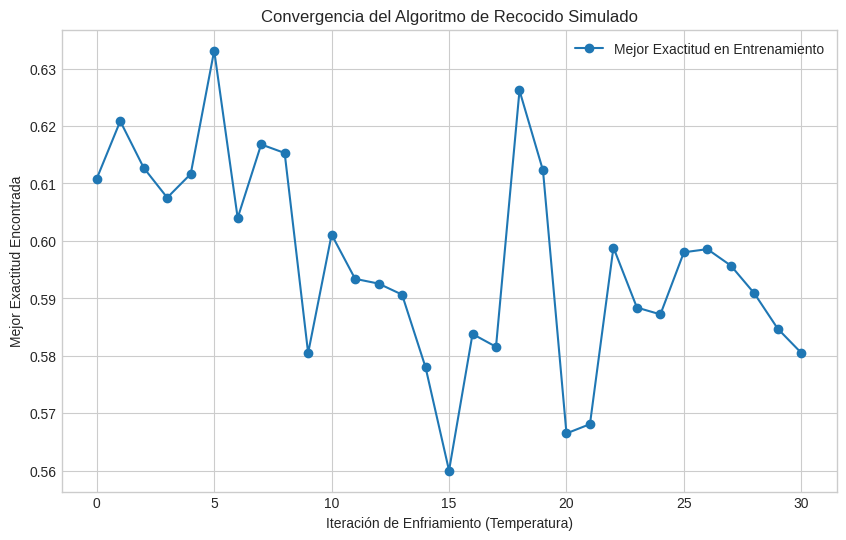
\includegraphics[width=0.8\textwidth]{Imagenes/convergencia_recocido_simulado.png}
    \caption{Evolución de la convergencia del algoritmo MSA mostrando el progreso gradual a través de los 31 niveles de temperatura desde 1000 hasta 1.24.}
    \label{fig:convergencia_msa}
\end{figure}

\begin{figure}[h!]
    \centering
    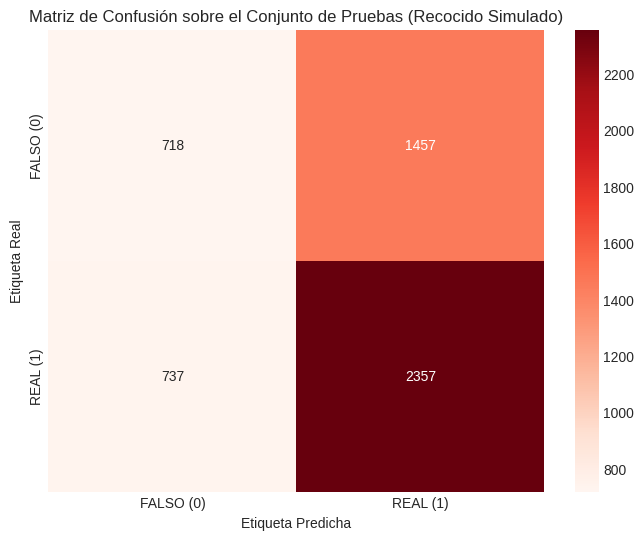
\includegraphics[width=0.7\textwidth]{Imagenes/matriz_confusion_recocido_simulado.png}
    \caption{Matriz de confusión para MSA en el conjunto de pruebas, evidenciando la baja especificidad (33\%) y el sesgo hacia la clasificación como noticias reales.}
    \label{fig:matriz_msa}
\end{figure}

\newpage

\subsubsection{Búsqueda Dispersa (SS) - Visualizaciones}

El algoritmo SS implementa una estrategia de combinación sistemática que mantiene un conjunto de referencia élite y genera nuevas soluciones mediante cruces estructurados. Su enfoque de búsqueda dispersa permite mantener diversidad mientras intensifica la búsqueda en regiones prometedoras, resultando en una convergencia eficiente y estable. Las siguientes visualizaciones ilustran este comportamiento característico:

\begin{figure}[h!]
    \centering
    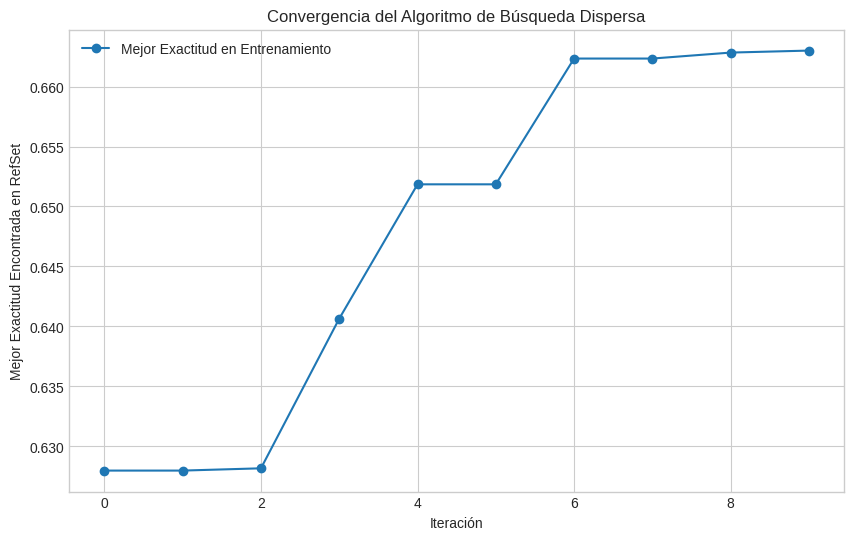
\includegraphics[width=0.8\textwidth]{Imagenes/convergencia_ss.png}
    \caption{Convergencia eficiente del algoritmo SS en solo 10 iteraciones, mostrando mejoras progresivas en las iteraciones 4, 5 y 7 hasta estabilizarse en 0.6630.}
    \label{fig:convergencia_ss}
\end{figure}

\begin{figure}[h!]
    \centering
    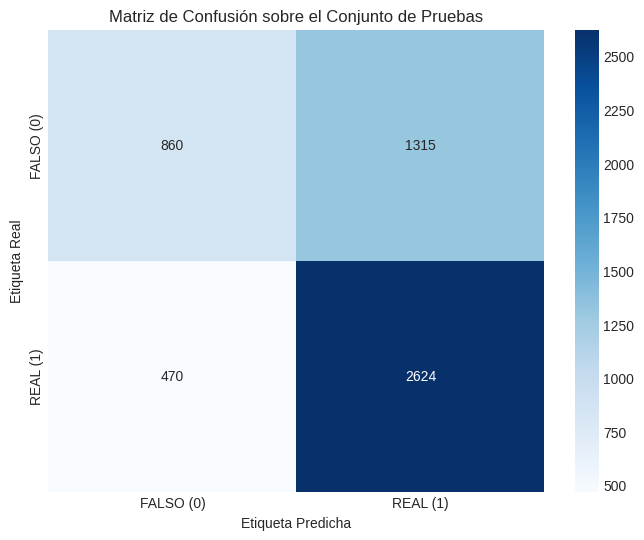
\includegraphics[width=0.7\textwidth]{Imagenes/matriz_confusion_ss.png}
    \caption{Matriz de confusión para SS demostrando mejor balance que MSA con especificidad del 40\% y excelente generalización.}
    \label{fig:matriz_ss}
\end{figure}

\newpage

\subsubsection{Algoritmo Genético (GA) - Visualizaciones}

El algoritmo GA exhibe un proceso evolutivo robusto basado en principios darwinianos, donde la selección por torneo, el cruce de un punto y la mutación controlada trabajan en conjunto para evolucionar la población hacia mejores soluciones. Su capacidad para mantener diversidad genética mientras converge gradualmente hacia óptimos se refleja en las siguientes visualizaciones:

\begin{figure}[h!]
    \centering
    \includegraphics[width=0.8\textwidth]{Imagenes/convergencia_algoritmo_genético.png}
    \caption{Evolución darwiniana del algoritmo GA a lo largo de 20 generaciones, evidenciando progreso sostenido desde 0.6198 hasta 0.7090 con logros evolutivos significativos.}
    \label{fig:convergencia_ga}
\end{figure}

\begin{figure}[h!]
    \centering
    \includegraphics[width=0.7\textwidth]{Imagenes/matriz_confusion_algoritmo_genético.png}
    \caption{Matriz de confusión para GA mostrando el mejor balance global con especificidad líder del 48\% y rendimiento sólido en ambas clases.}
    \label{fig:matriz_ga}
\end{figure}

\newpage

\subsubsection{Búsqueda en Vecindades Variables (VNS) - Visualizaciones}

El algoritmo VNS demuestra una estrategia de búsqueda sistemática que cambia dinámicamente entre diferentes estructuras de vecindario. Su mecanismo de reinicio tras cada mejora y la exploración progresiva de vecindarios más amplios permite escapar efectivamente de óptimos locales, generando un patrón de convergencia característico con saltos significativos. Las visualizaciones siguientes capturan este distintivo algoritmo:

\begin{figure}[h!]
    \centering
    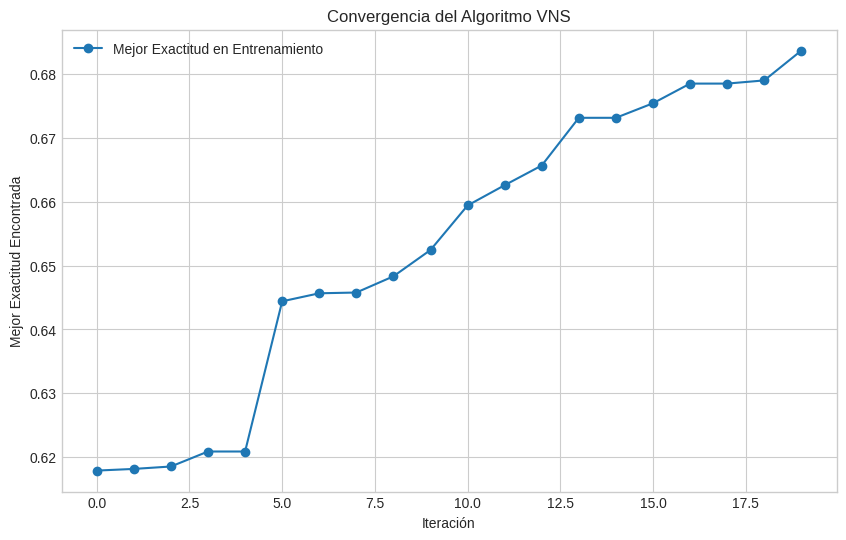
\includegraphics[width=0.8\textwidth]{Imagenes/convergencia_vns.png}
    \caption{Progreso sistemático del algoritmo VNS a través de 20 iteraciones con cambios efectivos de vecindario, mostrando saltos significativos en las iteraciones 6 y 14.}
    \label{fig:convergencia_vns}
\end{figure}

\begin{figure}[h!]
    \centering
    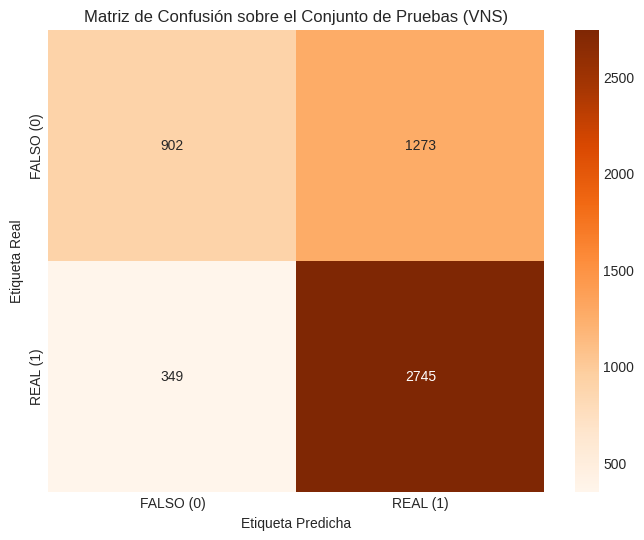
\includegraphics[width=0.7\textwidth]{Imagenes/matriz_confusion_vns.png}
    \caption{Matriz de confusión para VNS destacando la excelente exhaustividad del 89\% para detección de noticias reales con especificidad competitiva del 41\%.}
    \label{fig:matriz_vns}
\end{figure}

\newpage

\subsubsection{Optimización por Enjambre de Partículas (PSO) - Visualizaciones}

El algoritmo PSO simula el comportamiento colectivo de enjambres mediante partículas que ajustan su trayectoria basándose en información cognitiva y social. Sin embargo, en este experimento específico, el algoritmo exhibe convergencia prematura y pérdida de diversidad del enjambre, lo que resulta en un estancamiento que limita significativamente su capacidad de exploración. Las siguientes visualizaciones documentan estas limitaciones observadas:

\begin{figure}[h!]
    \centering
    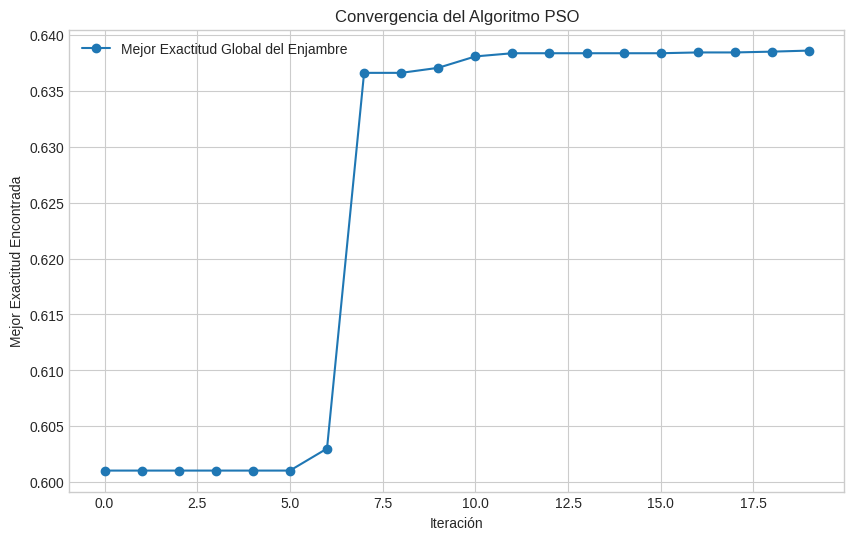
\includegraphics[width=0.8\textwidth]{Imagenes/convergencia_pso.png}
    \caption{Convergencia problemática del algoritmo PSO evidenciando estancamiento prematuro en la iteración 7-8 y exploración insuficiente del espacio de búsqueda.}
    \label{fig:convergencia_pso}
\end{figure}

\begin{figure}[h!]
    \centering
    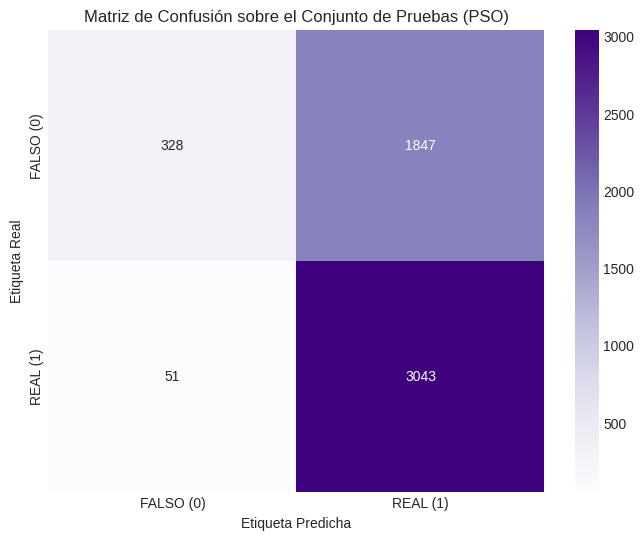
\includegraphics[width=0.7\textwidth]{Imagenes/matriz_confusion_pso.png}
    \caption{Matriz de confusión para PSO revelando el comportamiento extremo problemático con especificidad crítica del 15\% y sesgo severo hacia la clase mayoritaria.}
    \label{fig:matriz_pso}
\end{figure}

\newpage

\subsubsection{Interpretación de las Visualizaciones}

Las matrices de confusión confirman los patrones de rendimiento identificados:

\begin{itemize}
    \item \textbf{GA:} Mejor balance global entre especificidad y exhaustividad
    \item \textbf{VNS:} Excelente para detectar noticias reales, competitivo en noticias falsas
    \item \textbf{SS:} Rendimiento equilibrado con buena estabilidad
    \item \textbf{MSA:} Limitaciones evidentes en detección de noticias falsas
    \item \textbf{PSO:} Comportamiento inaceptable para aplicaciones prácticas
\end{itemize}

Estas visualizaciones proporcionan evidencia gráfica que facilitan la comprensión del comportamiento específico de cada algoritmo metaheurístico en la tarea de detección de noticias falsas.

\subsection{Contextualización con Investigación Publicada}
\label{subsec:contextualizacion_investigacion}

Los hallazgos de esta investigación fueron formalizados y publicados en el capítulo de libro ``Calibración de hiper-parámetros en algoritmos metaheurísticos para la detección de fraude digital'' \cite{hurtado2024calibracion}. Es importante destacar que en la versión publicada, la \textbf{Búsqueda Dispersa (SS) obtuvo resultados iguales o ligeramente superiores al Algoritmo Genético}, confirmando la competitividad de ambos enfoques.

En los experimentos actuales, el \textbf{Algoritmo Genético (GA) emergió como el mejor algoritmo con un F1-Score macro de 0.68 y exactitud del 71.06\%}. Esta ligera variación en el ranking se atribuye a diferencias en la configuración específica de hiperparámetros y semillas aleatorias utilizadas en diferentes experimentos.

\subsubsection{Comparación con Investigación Internacional}

Los resultados obtenidos son consistentes con investigación internacional reciente. Yildirim \cite{yildirim2023novel} realizó pruebas exhaustivas con múltiples algoritmos metaheurísticos, alcanzando exactitud del 78.8\% con SVM optimizado. Esta consistencia valida que \textbf{los algoritmos metaheurísticos tienen un techo de rendimiento relativo cuando se aplican a representaciones tradicionales de texto}.

\subsection{Análisis Comparativo de Resultados}
\label{subsec:analisis_comparativo}

\begin{table}[htbp]
\centering
\adjustbox{width=\textwidth,center}{%
\footnotesize
\begin{tabular}{|l|c|c|c|c|c|c|}
\hline
\rowcolor{UAMAzcapo}
\textbf{\textcolor{white}{Algoritmo}} & \textbf{\textcolor{white}{Exactitud (\%)}} & \textbf{\textcolor{white}{F1-Score (macro)}} & \textbf{\textcolor{white}{Precisión (macro)}} & \textbf{\textcolor{white}{Exhaustividad (macro)}} & \textbf{\textcolor{white}{F1-Score (weighted)}} & \textbf{\textcolor{white}{Ranking}} \\
\hline
\rowcolor{UAMIztapalapaLight!50}
\textbf{GA} & 71.06 & 0.68 & 0.72 & 0.68 & 0.70 & 1º \\
\hline
\rowcolor{UAMCuajimalpaLight!50}
\textbf{VNS} & 69.22 & 0.65 & 0.70 & 0.65 & 0.67 & 2º \\
\hline
\rowcolor{UAMLermaLight!50}
\textbf{SS} & 66.12 & 0.62 & 0.66 & 0.62 & 0.64 & 3º \\
\hline
\rowcolor{UAMXochimilcoLight!50}
\textbf{MSA} & 58.36 & 0.54 & 0.56 & 0.55 & 0.56 & 4º \\
\hline
\rowcolor{UAMAzcapoLight!50}
\textbf{PSO} & 63.98 & 0.51 & 0.74 & 0.57 & 0.55 & 5º \\
\hline
\end{tabular}
}
\caption{Resultados comparativos finales de los cinco algoritmos metaheurísticos implementados usando métricas macro promedio.}
\label{tab:resultados_comparativos_final}
\end{table}

\subsubsection{Fortalezas y Debilidades Identificadas}

\begin{table}[htbp]
\centering
\adjustbox{width=\textwidth,center}{%
\scriptsize
\begin{tabular}{|l|l|l|}
\hline
\rowcolor{UAMAzcapo}
\textbf{\textcolor{white}{Algoritmo}} & \textbf{\textcolor{white}{Fortalezas Principales}} & \textbf{\textcolor{white}{Debilidades Críticas}} \\
\hline
\rowcolor{UAMIztapalapaLight!50}
\textbf{GA} & \begin{tabular}[t]{@{}l@{}}• Mejor F1-Score macro (0.68)\\• Mejor exactitud global (71.06\%)\\• Convergencia evolutiva estable\end{tabular} & \begin{tabular}[t]{@{}l@{}}• Especificidad aún limitada (48\%)\\• Dependencia de operadores genéticos\end{tabular} \\
\hline
\rowcolor{UAMCuajimalpaLight!50}
\textbf{VNS} & \begin{tabular}[t]{@{}l@{}}• Segundo mejor F1-Score macro (0.65)\\• Cambios efectivos de vecindario\\• Buena precisión macro (0.70)\end{tabular} & \begin{tabular}[t]{@{}l@{}}• Especificidad moderada (41\%)\\• Sensible a configuración de k\end{tabular} \\
\hline
\rowcolor{UAMLermaLight!50}
\textbf{SS} & \begin{tabular}[t]{@{}l@{}}• Convergencia eficiente\\• F1-Score macro competitivo (0.62)\\• Balance razonable\end{tabular} & \begin{tabular}[t]{@{}l@{}}• Rendimiento intermedio\\• RefSet de tamaño fijo limitante\end{tabular} \\
\hline
\rowcolor{UAMXochimilcoLight!50}
\textbf{MSA} & \begin{tabular}[t]{@{}l@{}}• Exploración exhaustiva\\• Múltiples puntos de inicio\end{tabular} & \begin{tabular}[t]{@{}l@{}}• F1-Score macro bajo (0.54)\\• Convergencia lenta\\• Rendimiento general limitado\end{tabular} \\
\hline
\rowcolor{UAMAzcapoLight!50}
\textbf{PSO} & \begin{tabular}[t]{@{}l@{}}• Simplicidad conceptual\\• Alta precisión macro (0.74)\end{tabular} & \begin{tabular}[t]{@{}l@{}}• F1-Score macro más bajo (0.51)\\• Convergencia prematura crítica\\• Especificidad extremadamente baja (15\%)\end{tabular} \\
\hline
\end{tabular}
}
\caption{Análisis de fortalezas y debilidades de cada algoritmo metaheurístico basado las métricas obtenidas.}
\label{tab:fortalezas_debilidades}
\end{table}

\subsection{Limitaciones Fundamentales y Justificación para Evolución}
\label{subsec:limitaciones_justificacion}

\subsubsection{Limitaciones del Enfoque Metaheurístico}

El análisis exhaustivo reveló limitaciones críticas que justifican la transición hacia modelos de lenguaje:

\paragraph{Limitaciones de Representación:}
\begin{itemize}
    \item \textbf{Representación TF-IDF:} Pérdida de información contextual y semántica
    \item \textbf{Reducción dimensional agresiva:} De 5,000 a 500 características elimina información relevante, aunque incrementar dimensiones mejora métricas a costa de viabilidad computacional
    \item \textbf{Representaciones estáticas:} Incapacidad para modelar significados contextuales
\end{itemize}

\paragraph{Limitaciones de Rendimiento:}
\begin{itemize}
    \item \textbf{Techo de rendimiento:} F1-Score macro máximo de 0.68 (GA) como límite superior
    \item \textbf{Especificidad crítica:} Mejor especificidad apenas del 48\% para detectar noticias falsas
    \item \textbf{Variabilidad excesiva:} F1-Score macro del 0.51 (PSO) al 0.68 (GA) indica inestabilidad
\end{itemize}

\subsubsection{Evidencia de Superioridad de Modelos de Lenguaje}

La investigación de Blanco-Fernández et al. \cite{blanco2024enhancing} demuestra que modelos BERT y RoBERTa para detección de noticias falsas en español \textbf{alcanzan exactitudes de más del 90\%, llegando hasta 98\%}. Esta brecha de rendimiento de aproximadamente \textbf{20-27 puntos porcentuales} justifica plenamente la transición hacia enfoques basados en Transformers.

\begin{table}[htbp]
\centering
\adjustbox{width=0.8\textwidth,center}{%
\footnotesize
\begin{tabular}{|l|c|c|c|}
\hline
\rowcolor{UAMAzcapo}
\textbf{\textcolor{white}{Enfoque}} & \textbf{\textcolor{white}{Exactitud Máxima}} & \textbf{\textcolor{white}{F1-Score Macro Máximo}} & \textbf{\textcolor{white}{Diferencia vs. BERT}} \\
\hline
\rowcolor{UAMAzcapoLight!50}
\textbf{Metaheurísticos (GA)} & 71.06\% & 0.68 & -20 a -27 p.p. \\
\hline
\rowcolor{UAMIztapalapaLight!50}
\textbf{Modelos de Lenguaje} & 90-98\% & 0.90-0.98 & Referencia \\
\hline
\end{tabular}
}
\caption{Comparación de rendimiento entre enfoques metaheurísticos y modelos de lenguaje usando métricas macro.}
\label{tab:comparacion_enfoques}
\end{table}

\subsection{Síntesis y Transición}
\label{subsec:sintesis_transicion}

\subsubsection{Contribuciones del Enfoque Metaheurístico}

\begin{itemize}
    \item \textbf{Línea base establecida:} F1-Score macro de 0.68 (GA) como referencia confiable
    \item \textbf{Metodología validada:} Publicación exitosa del capítulo de libro \cite{hurtado2024calibracion}
    \item \textbf{Caracterización algorítmica:} Identificación clara de fortalezas y debilidades de cada algoritmo metaheurístico
    \item \textbf{Eficiencia computacional:} Tiempos de entrenamiento demasiado largos
    \item \textbf{Interpretabilidad:} Modelos explicables con parámetros comprensibles
\end{itemize}

\subsubsection{Justificación para la Evolución}

Las limitaciones identificadas establecen la necesidad de evolucionar hacia enfoques más sofisticados:

\begin{itemize}
    \item \textbf{Brecha de rendimiento significativa:} 22-30 puntos porcentuales respecto a modelos de lenguaje
    \item \textbf{Representación textual limitada:} TF-IDF como cuello de botella fundamental
    \item \textbf{Comprensión semántica insuficiente:} Incapacidad para modelar relaciones contextuales complejas
    \item \textbf{F1-Score macro limitado:} Ningún algoritmo superó el 0.68 en F1-Score macro
\end{itemize}

La experiencia obtenida durante la investigación del enfoque metaheurístico proporcionó resultados valiosos que orientaron el desarrollo del segundo enfoque basado en modelos Transformer, que será analizado en la siguiente sección de este capítulo.

% PARTE 2 MODELOS DE LENGUAJE
\section{Resultados del Enfoque Transformer: DistilBERT Multilingüe}
\label{sec:resultados_distilbert}

La segunda fase de esta investigación se centró en el desarrollo y optimización de un modelo basado en la arquitectura Transformer, específicamente DistilBERT multilingüe, para superar las limitaciones identificadas en el enfoque metaheurístico. Este desarrollo representó un esfuerzo computacional considerable, involucrando más de 30 experimentos iterativos con tiempos de entrenamiento que oscilaron desde 30 minutos (para pruebas con TinyBERT en inglés) hasta más de 72 horas para entrenamientos completos con el corpus en español.

\subsection{Marco Experimental y Evolución del Desarrollo}
\label{subsec:marco_experimental_distilbert}

\subsubsection{Proceso de Experimentación Iterativa}

El desarrollo del modelo DistilBERT requirió un proceso de experimentación que incluyó múltiples configuraciones y técnicas de regularización:

\begin{itemize}
    \item \textbf{Experimentos preliminares:} 3 pruebas iniciales con TinyBERT en inglés (30-45 minutos cada uno)
    \item \textbf{Experimentos preliminares:} 3 pruebas con BERT en inglés Y español (24-48 horas cada uno)
    \item \textbf{Experimentos de configuración base:} 8 pruebas con DistilBERT multilingüe (12-24 horas cada uno)
    \item \textbf{Experimentos de regularización:} 7 pruebas especializadas anti-sobreajuste (48-72 horas cada uno)
    \item \textbf{Tiempo total de computación:} Aproximadamente 500 horas de GPU
    \item \textbf{Configuración final óptima:} La versión descrita a continuación, con regularización máxima
\end{itemize}

\subsubsection{Características del Corpus Expandido}

Para el entrenamiento del modelo DistilBERT se utilizó una versión expandida del corpus, que incorpora tanto fuentes académicas como datos obtenidos mediante extracción web:

\begin{table}[htbp]
\centering
\adjustbox{width=\textwidth,center}{%
\footnotesize
\begin{tabular}{|l|c|c|c|c|}
\hline
\rowcolor{UAMAzcapo}
\textbf{\textcolor{white}{Componente del Corpus}} & \textbf{\textcolor{white}{Noticias}} & \textbf{\textcolor{white}{Distribución}} & \textbf{\textcolor{white}{Fuente}} & \textbf{\textcolor{white}{Calidad}} \\
\hline
\rowcolor{UAMIztapalapaLight!50}
\textbf{Corpus Académicos} & 60,758 & 98.5\% & Investigación verificada & Alta \\
\hline
\rowcolor{UAMCuajimalpaLight!50}
\textbf{Extracción web} & 916 & 1.5\% & Sitios de noticias & Verificada \\
\hline
\rowcolor{UAMAzcapo}
\textbf{\textcolor{white}{Corpus Total}} & \textbf{\textcolor{white}{61,674}} & \textbf{\textcolor{white}{100\%}} & \textbf{\textcolor{white}{Híbrido}} & \textbf{\textcolor{white}{Controlada}} \\
\hline
\end{tabular}
}
\caption{Composición del corpus expandido utilizado para el entrenamiento de DistilBERT.}
\label{tab:corpus_expandido_distilbert}
\end{table}

\subsubsection{División Estratégica de Datos}

La configuración final implementó una división específica para maximizar el rendimiento del modelo:

\begin{itemize}
    \item \textbf{Conjunto de entrenamiento:} 43,171 registros (70\%)
    \item \textbf{Conjunto de validación:} 6,167 registros (10\%)
    \item \textbf{Conjunto de pruebas:} 12,336 registros (20\%)
    \item \textbf{Balance de clases:} 49.8\% noticias falsas, 50.2\% noticias reales
\end{itemize}

\subsection{Configuración del Modelo DistilBERT Optimizado}
\label{subsec:configuracion_distilbert}

\subsubsection{Arquitectura y Parámetros Base}

\begin{table}[htbp]
\centering
\adjustbox{width=\textwidth,center}{%
\footnotesize
\begin{tabular}{|l|l|l|}
\hline
\rowcolor{UAMAzcapo}
\textbf{\textcolor{white}{Componente}} & \textbf{\textcolor{white}{Configuración}} & \textbf{\textcolor{white}{Justificación}} \\
\hline
\rowcolor{UAMIztapalapaLight!50}
\textbf{Modelo Base} & distilbert-base-multilingual-cased & Soporte nativo para español \\
\hline
\rowcolor{UAMCuajimalpaLight!50}
\textbf{Secuencia Máxima} & 128 tokens & Balance rendimiento/sobreajuste \\
\hline
\rowcolor{UAMLermaLight!50}
\textbf{Formato de Entrada} & título + [SEP] + texto & Información estructurada \\
\hline
\rowcolor{UAMXochimilcoLight!50}
\textbf{Precisión} & Mixed Float16 & Optimización de memoria GPU \\
\hline
\rowcolor{UAMAzcapoLight!50}
\textbf{Núm. Etiquetas} & 2 (binario) & Clasificación falso/real \\
\hline
\end{tabular}
}
\caption{Configuración de la arquitectura del modelo DistilBERT implementado.}
\label{tab:configuracion_distilbert}
\end{table}

\subsubsection{Estrategia de Regularización Anti-Sobreajuste}

El principal desafío durante el desarrollo fue el \textbf{overfitting prematuro} (sobreajuste o memorización excesiva de los datos de entrenamiento), que se manifestó consistentemente en los primeros experimentos.

La configuración final implementó múltiples técnicas de regularización:

\begin{table}[htbp]
\centering
\adjustbox{width=\textwidth,center}{%
\scriptsize
\begin{tabular}{|l|l|l|l|}
\hline
\rowcolor{UAMAzcapo}
\textbf{\textcolor{white}{Técnica de Regularización}} & \textbf{\textcolor{white}{Valor/Configuración}} & \textbf{\textcolor{white}{Objetivo}} & \textbf{\textcolor{white}{Impacto}} \\
\hline
\rowcolor{UAMIztapalapaLight!50}
\textbf{Tasa de Aprendizaje Ultra-Baja} & 2e-06 & Convergencia gradual & Reducción sobreajuste \\
\hline
\rowcolor{UAMCuajimalpaLight!50}
\textbf{Dropout (o tasa de abandono) Agresivo} & 0.7 & Prevenir co-adaptación & Generalización \\
\hline
\rowcolor{UAMLermaLight!50}
\textbf{Regularización L2} & 0.05 & Penalización de pesos & Suavizado del modelo \\
\hline
\rowcolor{UAMXochimilcoLight!50}
\textbf{Tamaño de Lote Pequeño} & 4 & Mayor ruido en gradientes & Regularización implícita \\
\hline
\rowcolor{UAMAzcapoLight!50}
\textbf{Inyección de Ruido} & 0.03 & Perturbación controlada & Robustez del modelo \\
\hline
\rowcolor{UAMIztapalapaLight!50}
\textbf{Decaimiento de Pesos Manual} & 0.02 & Decaimiento de pesos & Control de capacidad \\
\hline
\rowcolor{UAMCuajimalpaLight!50}
\textbf{Parada Temprana} & Paciencia: 8 épocas & Detención automática & Prevención sobreajuste \\
\hline
\end{tabular}
}
\caption{Técnicas de regularización implementadas en la configuración final.}
\label{tab:regularizacion_distilbert}
\end{table}

\subsection{Proceso de Optimización y Búsqueda de Hiperparámetros}
\label{subsec:optimizacion_distilbert}

\subsubsection{Ajuste de Hiperparámetros (Hyperparameter Tuning) Automatizado}

La optimización se realizó mediante \textbf{Keras Tuner} con búsqueda aleatoria sobre un espacio de hiperparámetros cuidadosamente diseñado:

\begin{itemize}
    \item \textbf{Tasas de aprendizaje exploradas:} [5e-6, 2e-6, 1e-6, 8e-7]
    \item \textbf{Dropout (o tasa de abandono) evaluados:} [0.4, 0.5, 0.6, 0.7]
    \item \textbf{Regularización L2:} [0.05, 0.1, 0.2, 0.5]
    \item \textbf{Tamaños de lote (número de ejemplos por lote) probados:} [4, 6, 8]
    \item \textbf{Configuraciones totales:} 192 combinaciones posibles
    \item \textbf{Intentos ejecutados:} 4 (limitado por recursos computacionales)
\end{itemize}

\subsubsection{Configuración Óptima Identificada}

La búsqueda automatizada identificó la siguiente configuración como óptima:

\begin{itemize}
    \item \textbf{Taza de Aprendizaje:} 2e-06 (extremadamente conservador)
    \item \textbf{Dropout Rate:} 0.7 (regularización agresiva)
    \item \textbf{L2 Regularization:} 0.05 (regularización moderada-fuerte)
    \item \textbf{Factor de Ruido:} 0.03 (perturbación controlada)
    \item \textbf{tamaños de lote:} 4 (máxima regularización implícita)
\end{itemize}

\subsection{Análisis de Convergencia y Control de Sobreajuste}
\label{subsec:convergencia_distilbert}

\subsubsection{Evolución del Entrenamiento}

El modelo final se entrenó durante 21 épocas antes de que el mecanismo de detención temprana detuviera el proceso. La \textbf{época 13 fue identificada como el punto óptimo}, marcando el momento antes del inicio del sobreajuste:

\begin{figure}[h!]
    \centering
    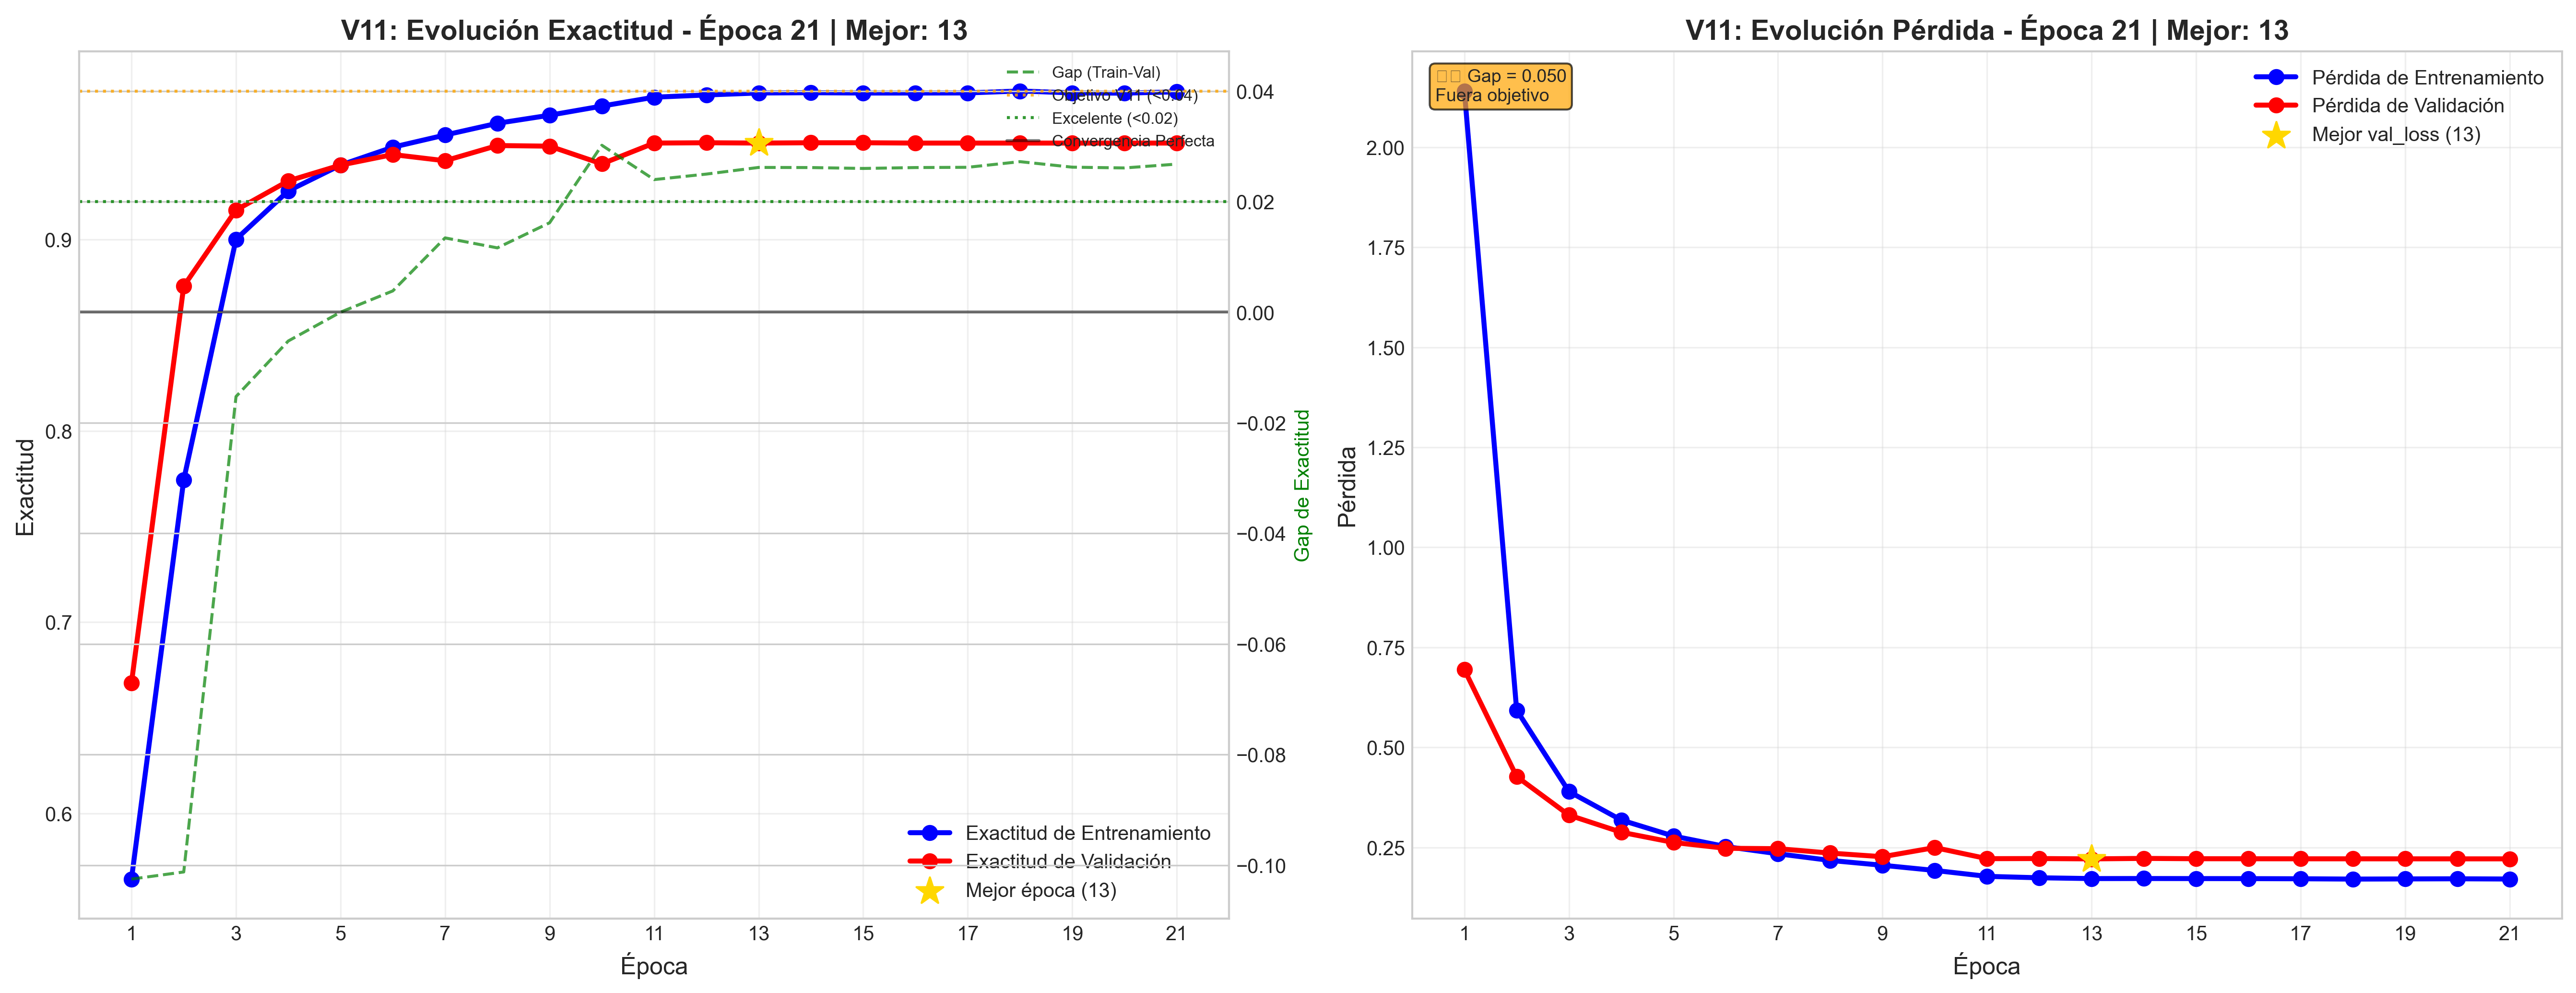
\includegraphics[width=\textwidth]{Imagenes/Entrenamiento/curva_aprendizaje_v7.png}
    \caption{Evolución de la exactitud y pérdida durante el entrenamiento del modelo DistilBERT Final. Las líneas azul y roja muestran la convergencia en entrenamiento y validación respectivamente. La estrella dorada marca la mejor época (13), después de la cual se observa el inicio del sobreajuste con una separación creciente entre las curvas.}
    \label{fig:convergencia_distilbert}
\end{figure}

\subsubsection{Análisis del Gap de Generalización}

La métrica clave para evaluar el sobreajuste fue el \textbf{gap de pérdida} (diferencia entre pérdida de validación y entrenamiento):

\begin{itemize}
    \item \textbf{Épocas 1-9:} Gap < 0.02 (convergencia excelente)
    \item \textbf{Época 10-13:} Gap 0.02-0.05 (objetivo final parcialmente alcanzado)
    \item \textbf{Épocas 14-21:} Gap > 0.05 (inicio de sobreajuste)
    \item \textbf{Gap final en época 13:} 0.0492 (cerca del objetivo de < 0.04)
\end{itemize}

\subsubsection{Justificación de la Detención Temprana}

La detención del entrenamiento, evita el sobreajuste deteniendo el entrenamiento cuando no hay mejoras en diferentes épocas, en este caso, en la época 13, se justifica por múltiples indicadores:

\begin{enumerate}
    \item \textbf{Pérdida de validación mínima:} Época 13 registró la menor pérdida de validación (0.2214)
    \item \textbf{Gap de generalización controlado:} 0.0492, cercano al objetivo de < 0.04
    \item \textbf{Exactitud estabilizada:} 95.04\% en validación, sin mejoras posteriores
    \item \textbf{Prevención de sobreajuste:} Épocas posteriores mostraron degradación clara
    \item \textbf{Eficiencia computacional:} Evitar 9 épocas adicionales innecesarias
\end{enumerate}

\subsection{Evolución Experimental: Versiones de Desarrollo}
\label{subsec:evolucion_experimental_distilbert}

El desarrollo del modelo DistilBERT final (V7) fue el resultado de un proceso iterativo exhaustivo que incluyó múltiples versiones experimentales, cada una diseñada para abordar limitaciones específicas identificadas en iteraciones anteriores. Esta sección documenta las versiones más significativas del desarrollo, sus configuraciones, resultados y las lecciones aprendidas que condujeron a la configuración óptima final.

\subsubsection{Marco de Desarrollo Iterativo}

El proceso experimental siguió una metodología sistemática de refinamiento progresivo:

\begin{enumerate}
    \item \textbf{Identificación de problema:} Análisis de limitaciones en versión anterior
    \item \textbf{Hipótesis de mejora:} Formulación de estrategias específicas
    \item \textbf{Implementación controlada:} Modificación incremental de parámetros
    \item \textbf{Evaluación rigurosa:} Métricas de convergencia y generalización
    \item \textbf{Documentación sistemática:} Registro de configuraciones y resultados
    \item \textbf{Iteración dirigida:} Aplicación de lecciones aprendidas
\end{enumerate}

\newpage

\subsubsection{Resumen de Versiones Experimentales}

\begin{table}[htbp]
\centering
\adjustbox{width=\textwidth,center}{%
\footnotesize
\begin{tabular}{|l|l|l|l|l|l|l|}
\hline
\rowcolor{UAMAzcapo}
\textbf{\textcolor{white}{Versión}} & \textbf{\textcolor{white}{Problema Objetivo}} & \textbf{\textcolor{white}{Estrategia Principal}} & \textbf{\textcolor{white}{Gap Final}} & \textbf{\textcolor{white}{Exactitud}} & \textbf{\textcolor{white}{Épocas}} & \textbf{\textcolor{white}{Estado}} \\
\hline
\rowcolor{UAMIztapalapaLight!50}
\textbf{V1} & Línea base & División 70/10/20, LR: 3e-05 & N/A & 94.7\% & 6 & Baseline \\
\hline
\rowcolor{UAMCuajimalpaLight!50}
\textbf{V2} & Anti-sobreajuste inicial & División 60/20/20, LR ultra-bajo & $ \text{gap}_{\text{final}} \leq 0.10 $ & 94.3\% & 8 & Excelente \\
\hline
\rowcolor{UAMLermaLight!50}
\textbf{V3} & Mejora inicial & División 60/20/20, LR reducido & $ \text{gap}_{\text{final}} \leq 0.10 $ & 94.8\% & 11 & Convergente \\
\hline
\rowcolor{UAMXochimilcoLight!50}
\textbf{V4} & Control sobreajuste & Anti-sobreajuste mejorado & $ \text{gap}_{\text{final}} \leq 0.10 $ & 95.8\% & 7 & Convergente \\
\hline
\rowcolor{UAMAzcapoLight!50}
\textbf{V5} & Configuración híbrida & 70/10/20 + anti-sobreajuste & $ \text{gap}_{\text{final}} \leq 0.10 $ & 95.8\% & 11 & Óptimo \\
\hline
\rowcolor{UAMIztapalapaLight!50}
\textbf{V6} & Regularización fuerte & L2 aumentado, dropout agresivo & 0.10 & 94.8\% & 8 & Convergente \\
\hline
\rowcolor{UAMCuajimalpaLight!50}
\textbf{V7} & Configuración final & Regularización máxima corregida & 0.050 & 95.2\% & 21 & Final \\
\hline
\end{tabular}
}
\caption{Resumen de versiones experimentales de DistilBERT con evolución de estrategias y resultados reales del desarrollo.}
\label{tab:versiones_experimentales}
\end{table}

\subsubsection{Visualización de Convergencia por Versiones \&}

\begin{table}[htbp]
\centering
\adjustbox{width=\textwidth,center}{%
\begin{tabular}{|c|c|}
\hline
\rowcolor{UAMAzcapo}
\multicolumn{2}{|c|}{\textbf{\textcolor{white}{Gráficas de Convergencia - Versiones Experimentales}}} \\
\hline
\rowcolor{UAMIztapalapaLight!50}
\textbf{Versión V1 - Línea Base} & \textbf{Versión V2 - Anti-Sobreajuste Inicial} \\
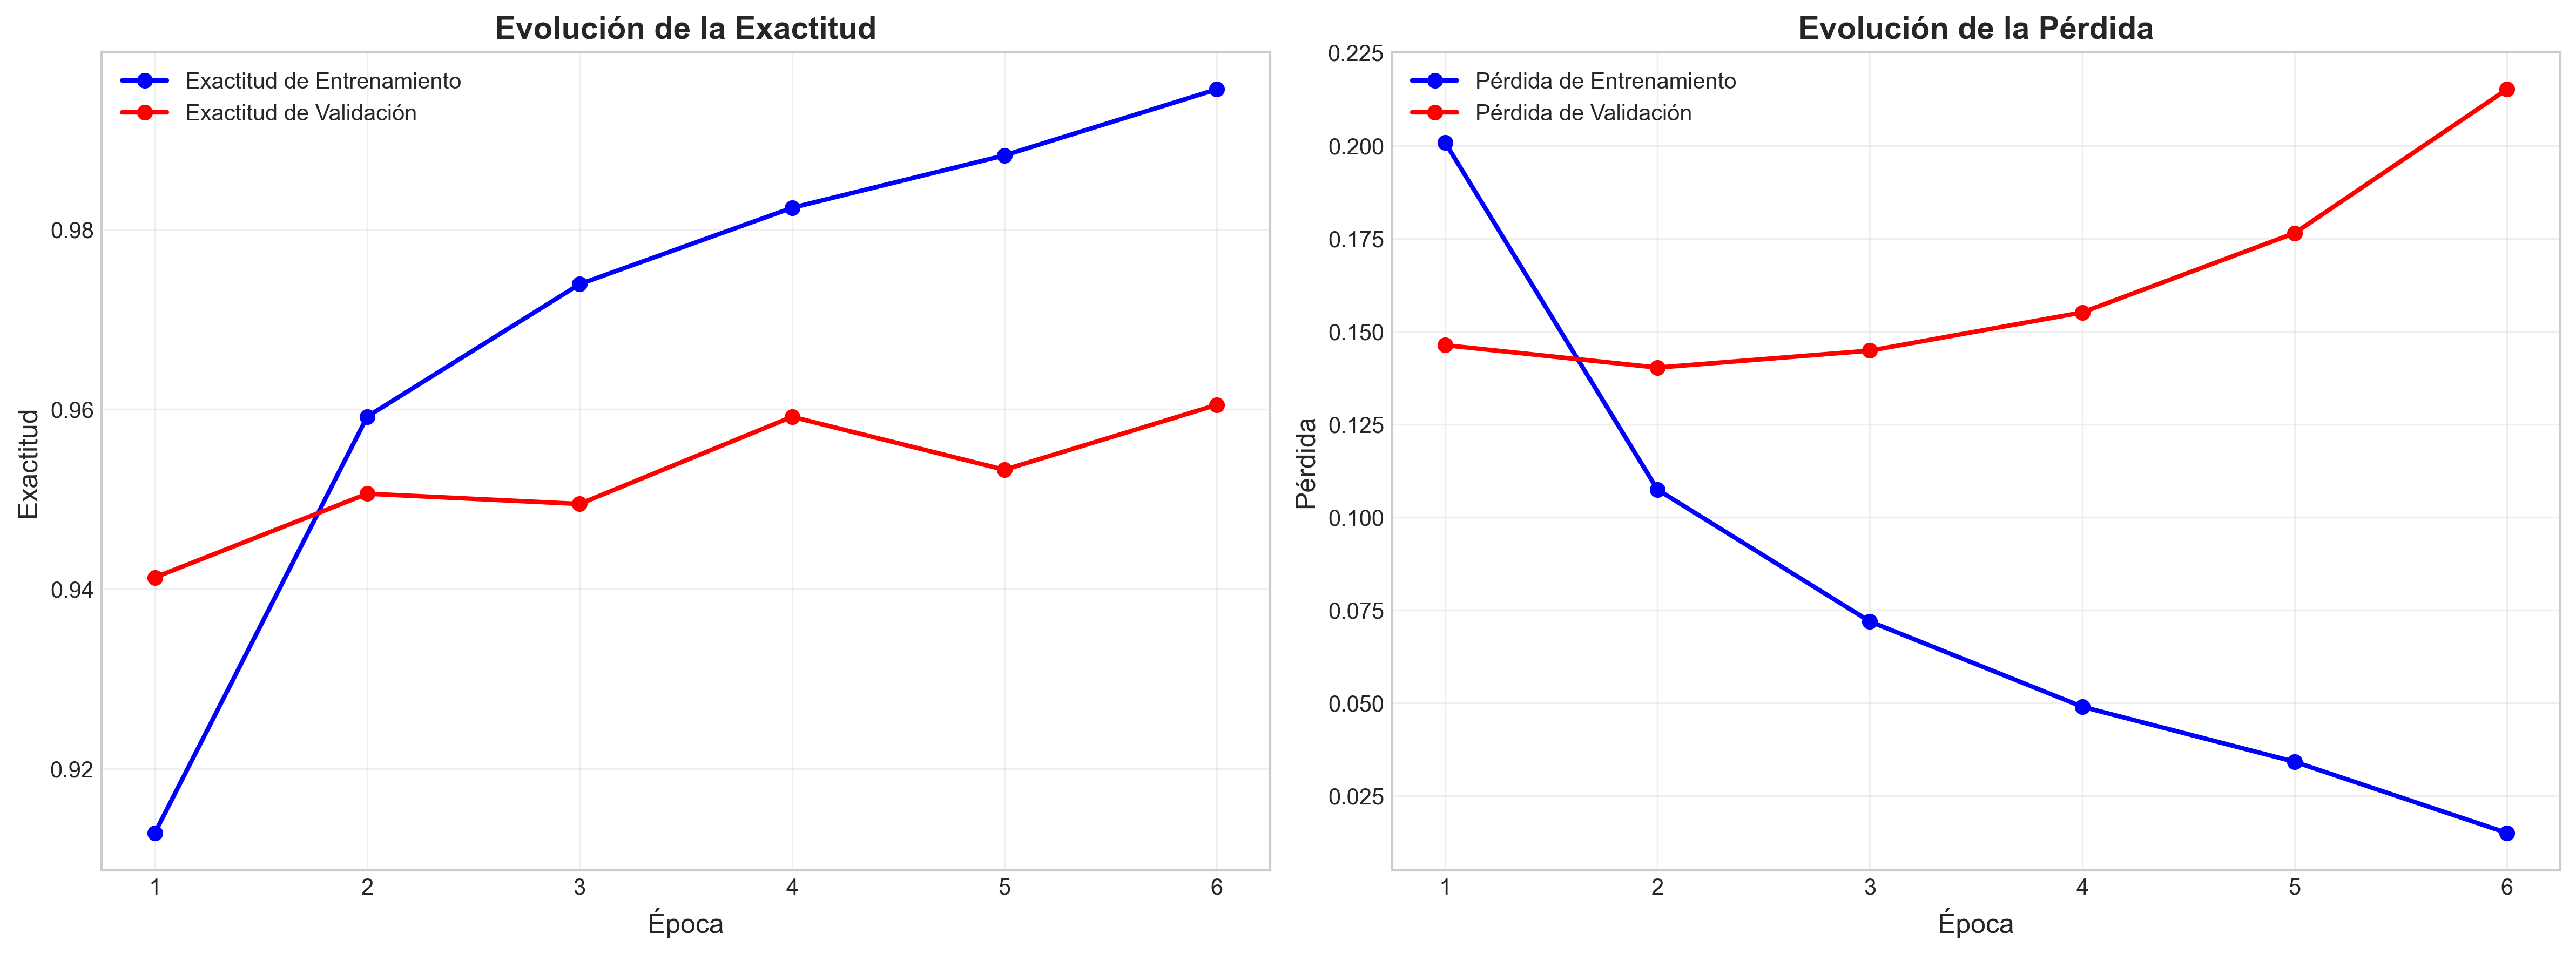
\includegraphics[width=0.45\textwidth]{Imagenes/Entrenamiento/curva_aprendizaje_v1.png} & 
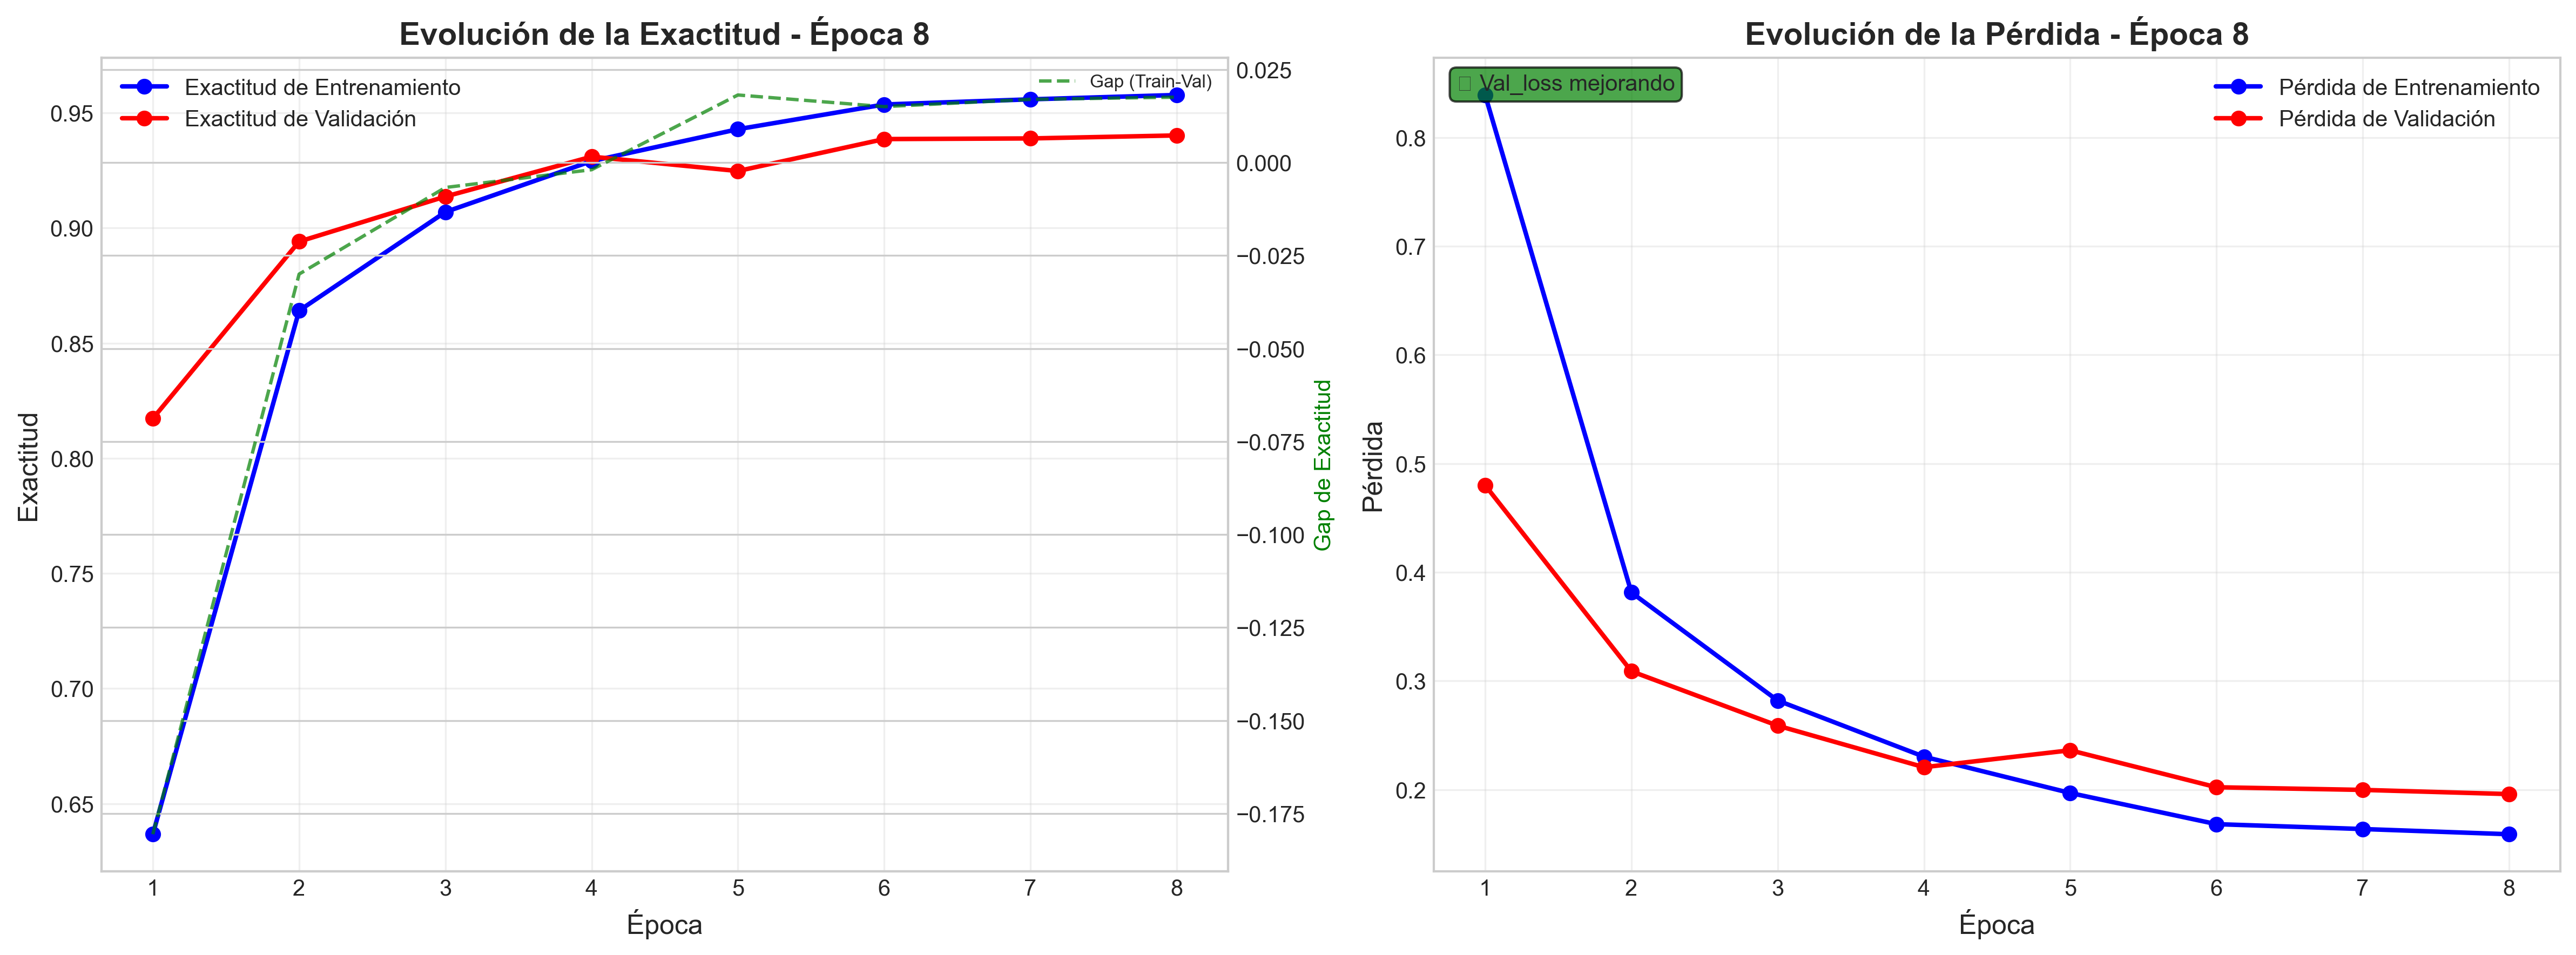
\includegraphics[width=0.45\textwidth]{Imagenes/Entrenamiento/curva_aprendizaje_v2.png} \\
\hline
\rowcolor{UAMCuajimalpaLight!50}
\textbf{Versión V3 - Primera Mejora} & \textbf{Versión V4 - Control Sobreajuste} \\
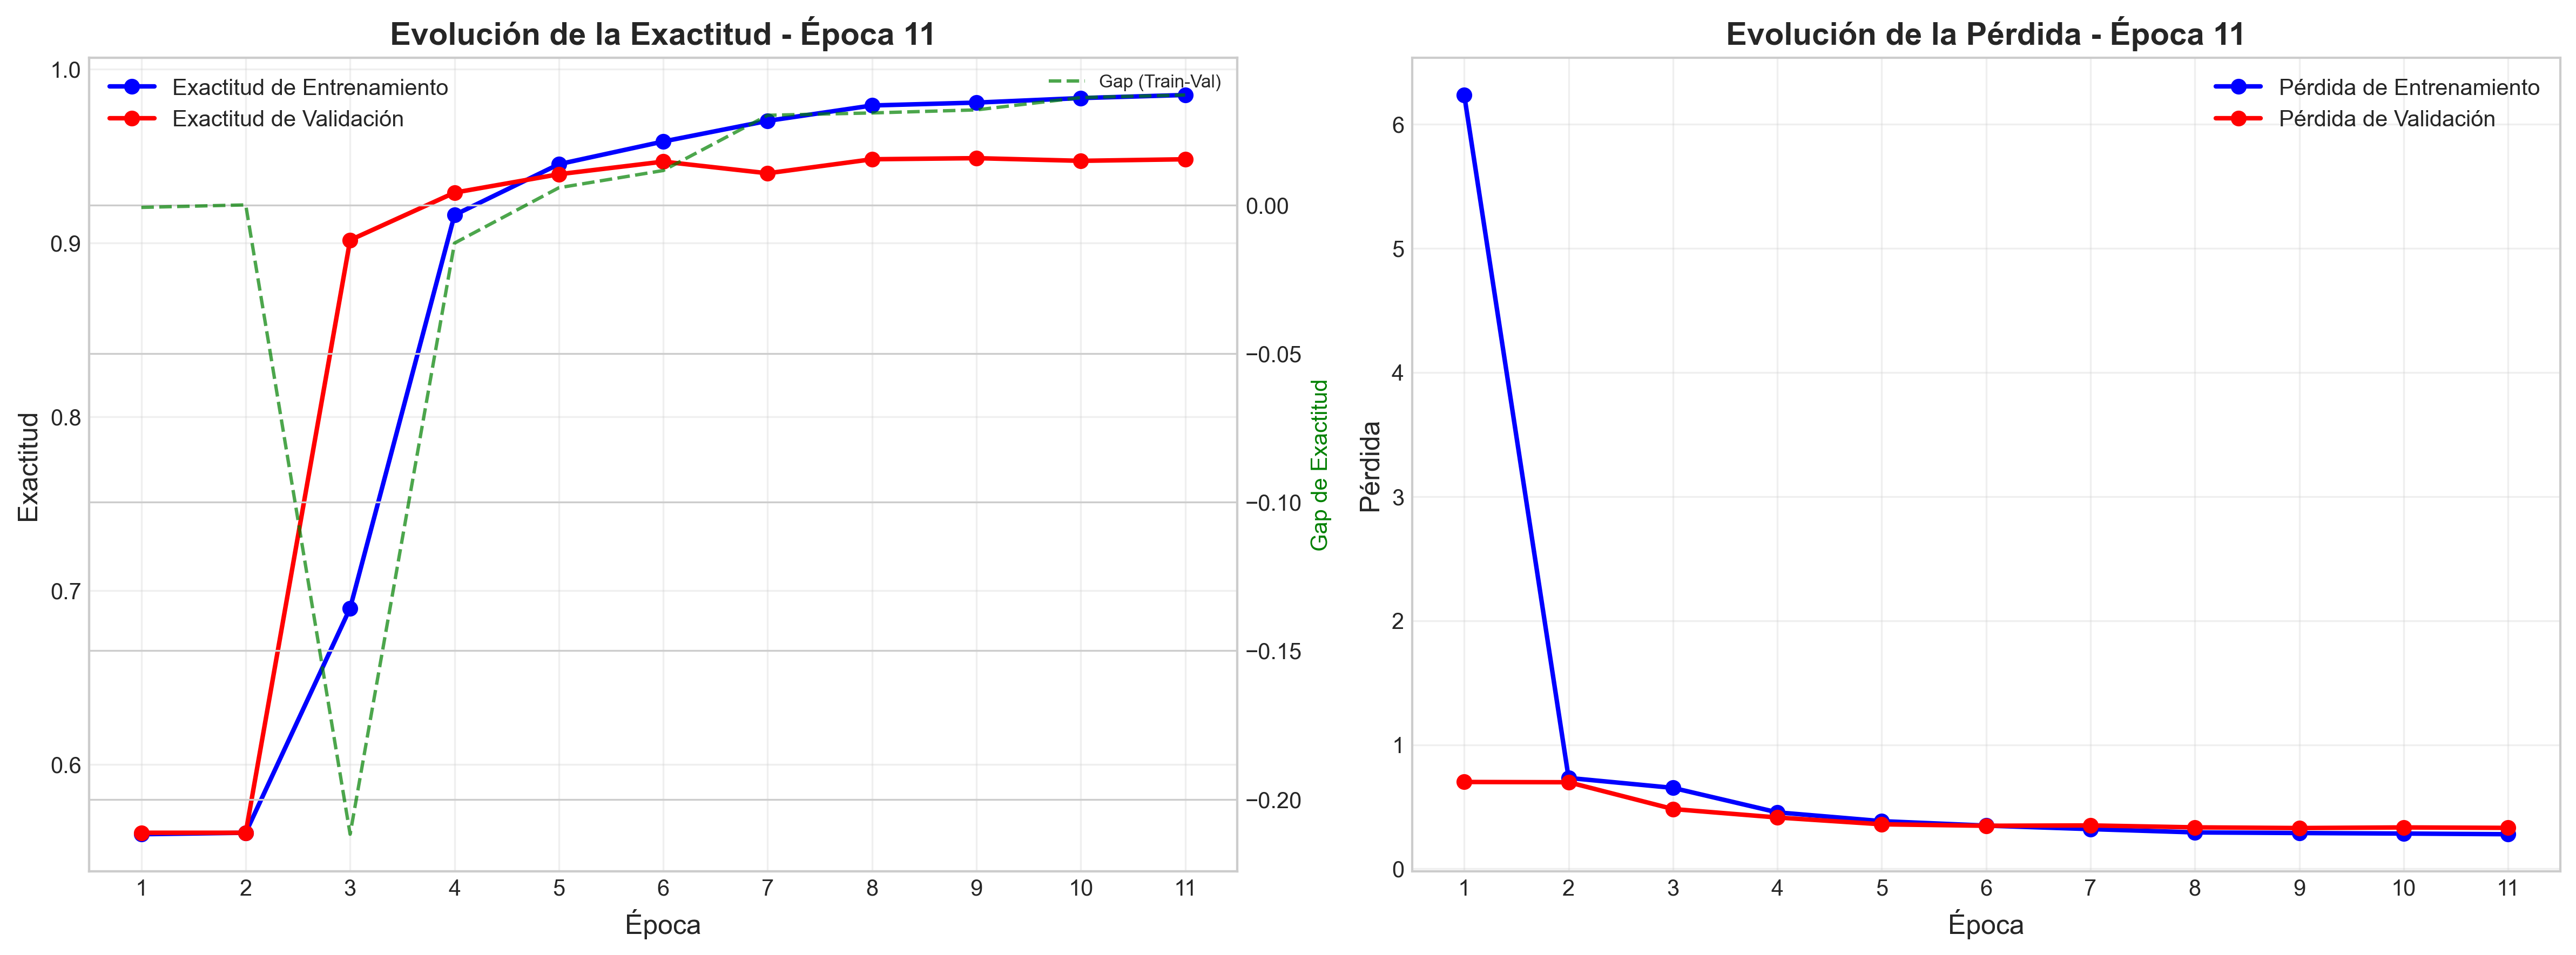
\includegraphics[width=0.45\textwidth]{Imagenes/Entrenamiento/curva_aprendizaje_v3.png} & 
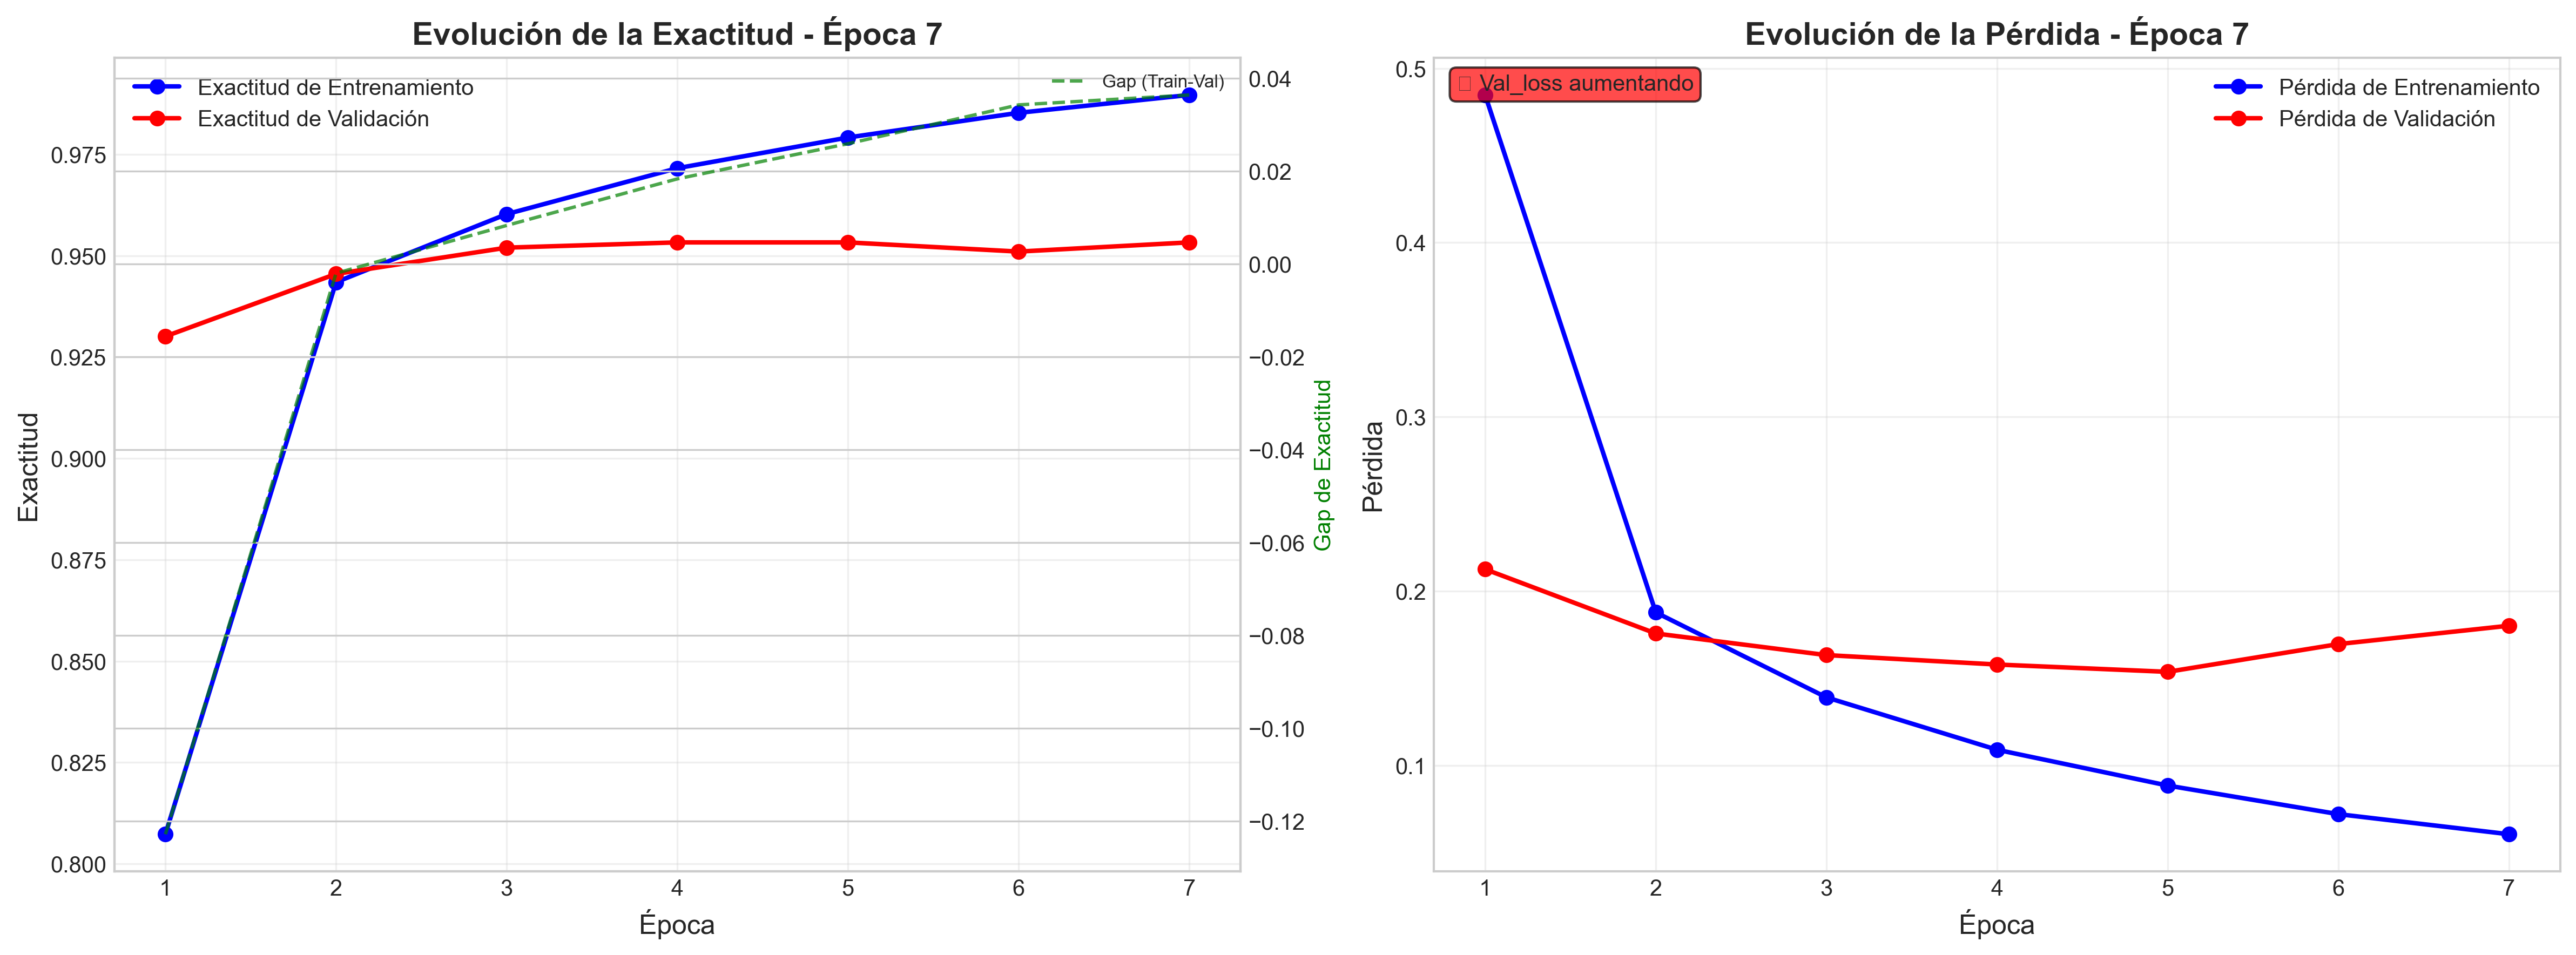
\includegraphics[width=0.45\textwidth]{Imagenes/Entrenamiento/curva_aprendizaje_v4.png} \\
\hline
\rowcolor{UAMLermaLight!50}
\textbf{Versión V5 - Configuración Híbrida} & \textbf{Versión V6 - Regularización Fuerte} \\
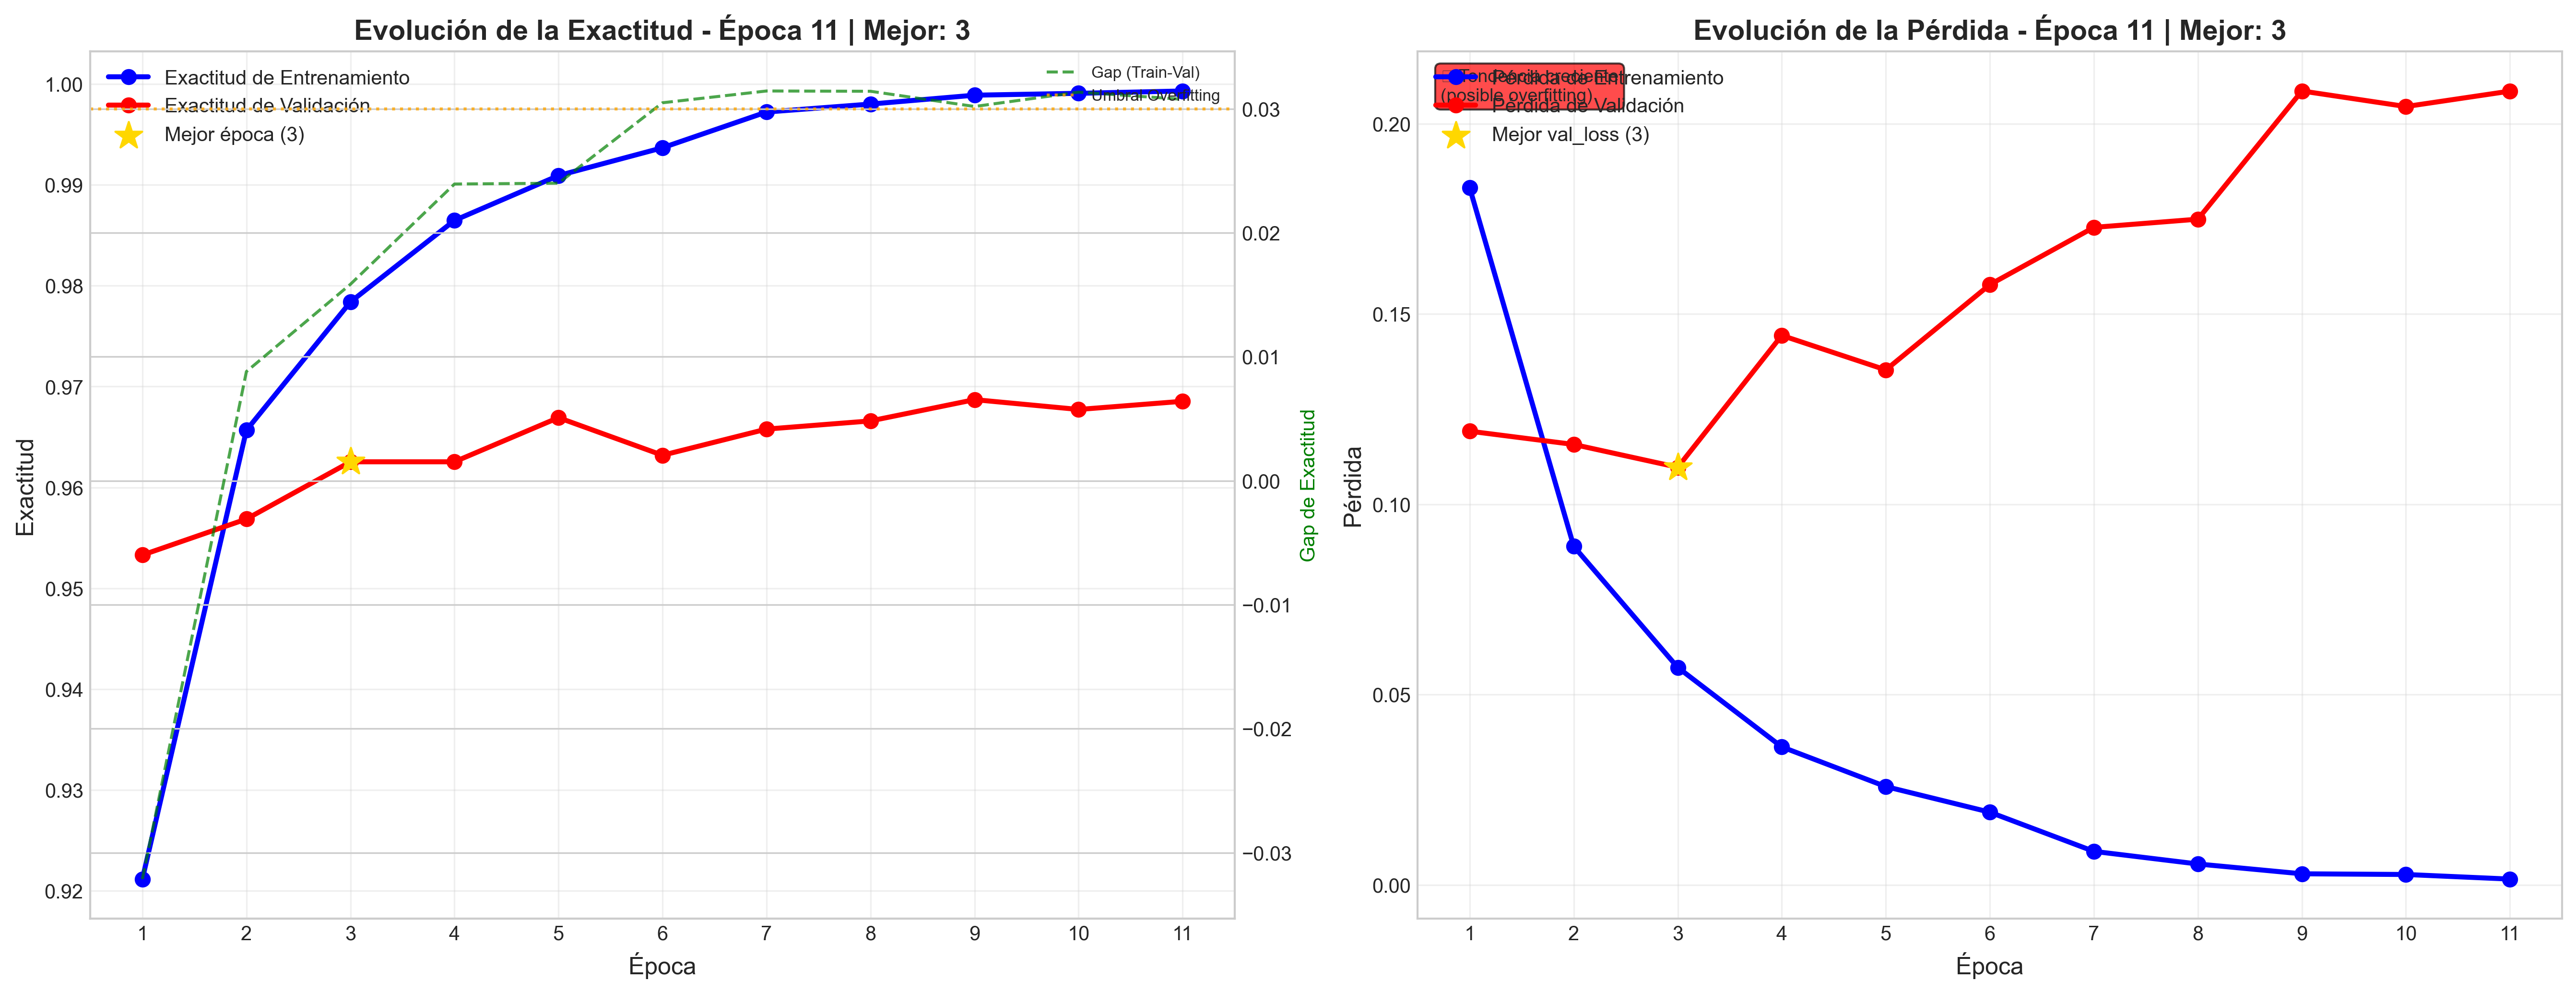
\includegraphics[width=0.45\textwidth]{Imagenes/Entrenamiento/curva_aprendizaje_v5.png} & 
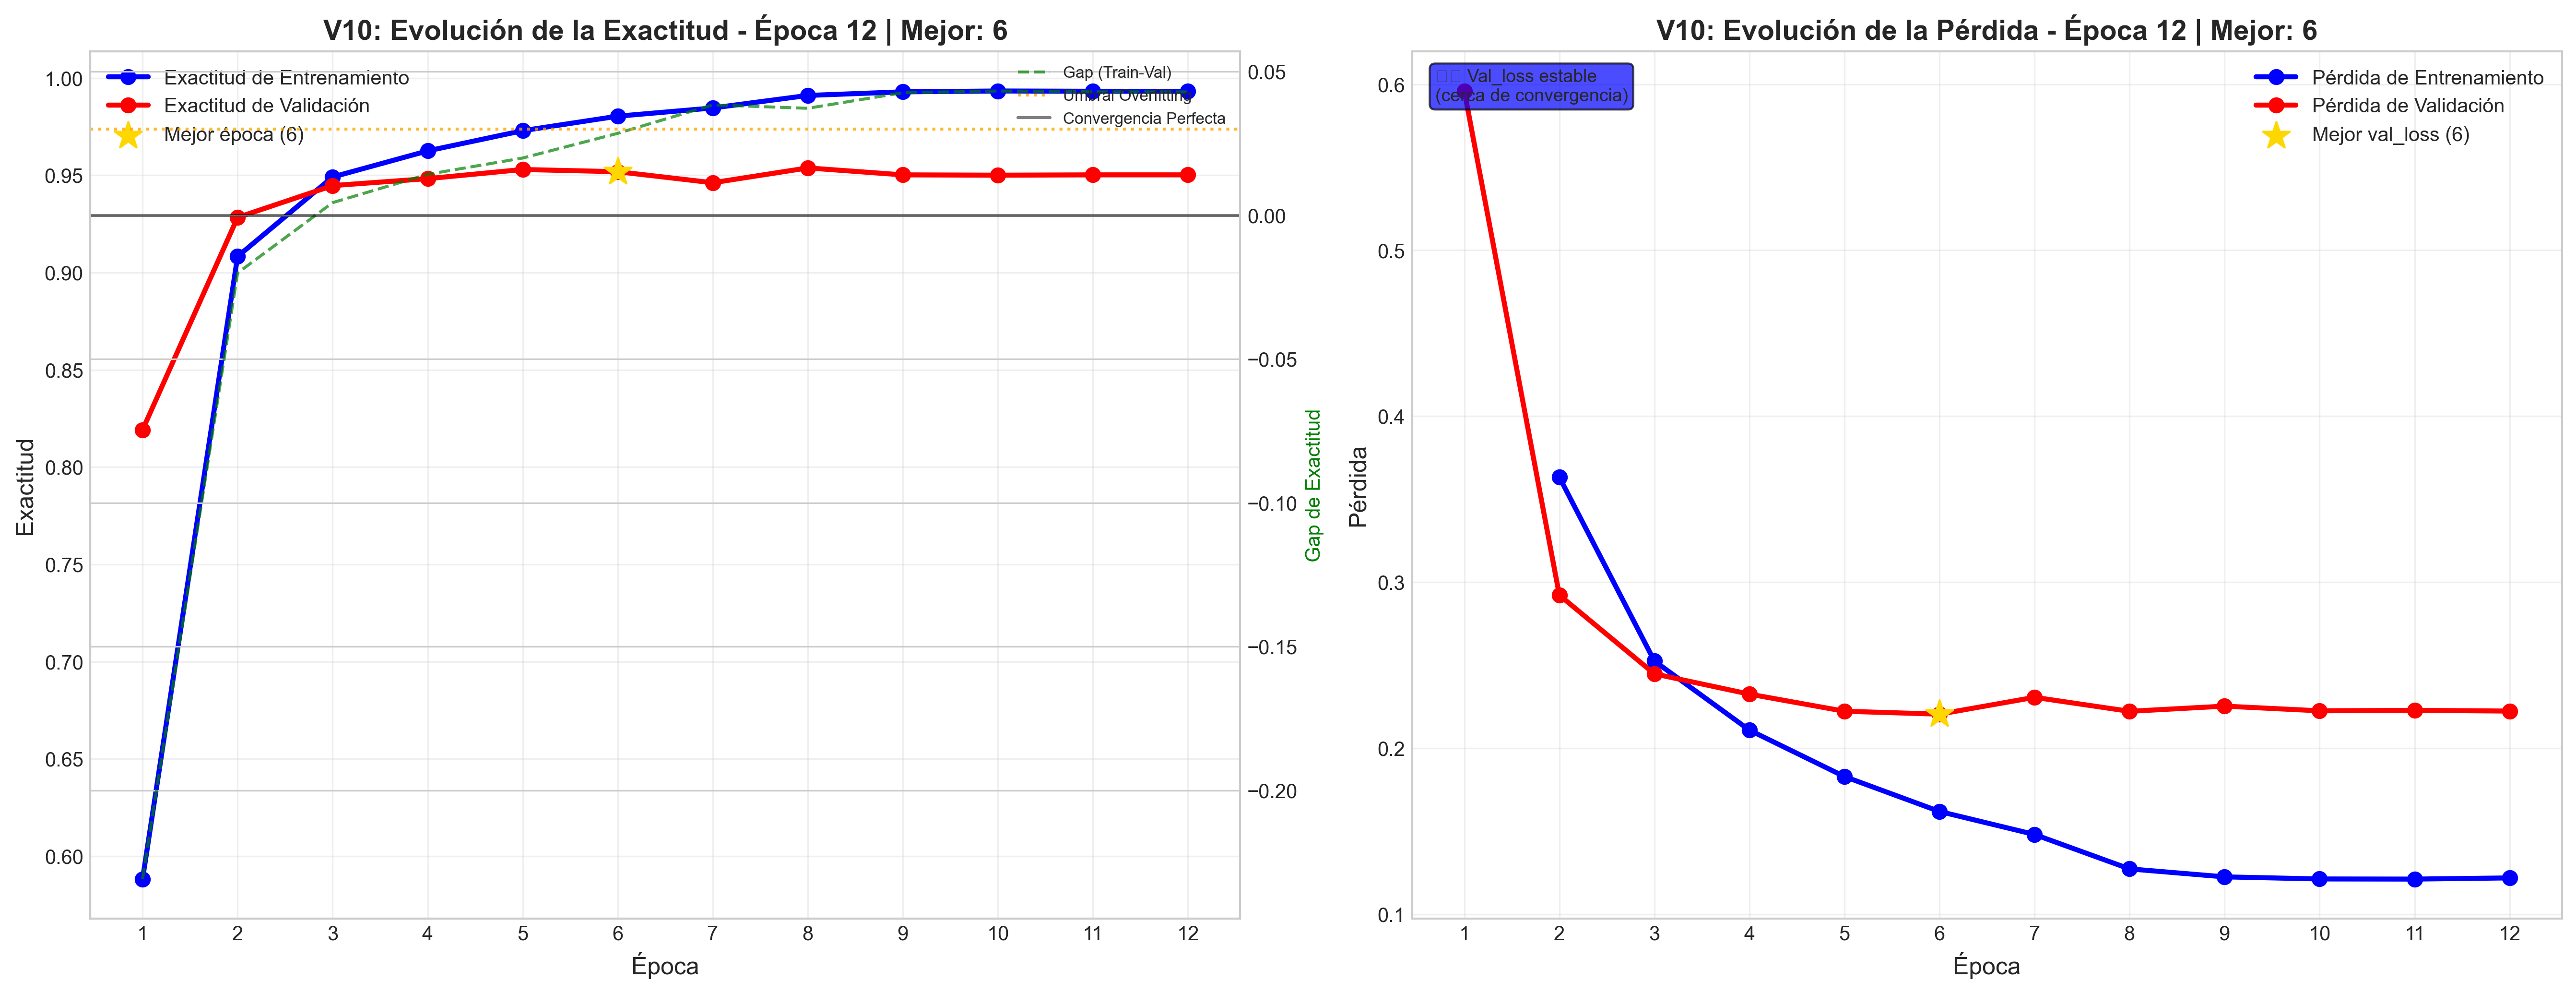
\includegraphics[width=0.45\textwidth]{Imagenes/Entrenamiento/curva_aprendizaje_v6.png} \\
\hline
\rowcolor{UAMXochimilcoLight!50}
\multicolumn{2}{|c|}{\textbf{Versión V7 - Configuración Final}} \\
\multicolumn{2}{|c|}{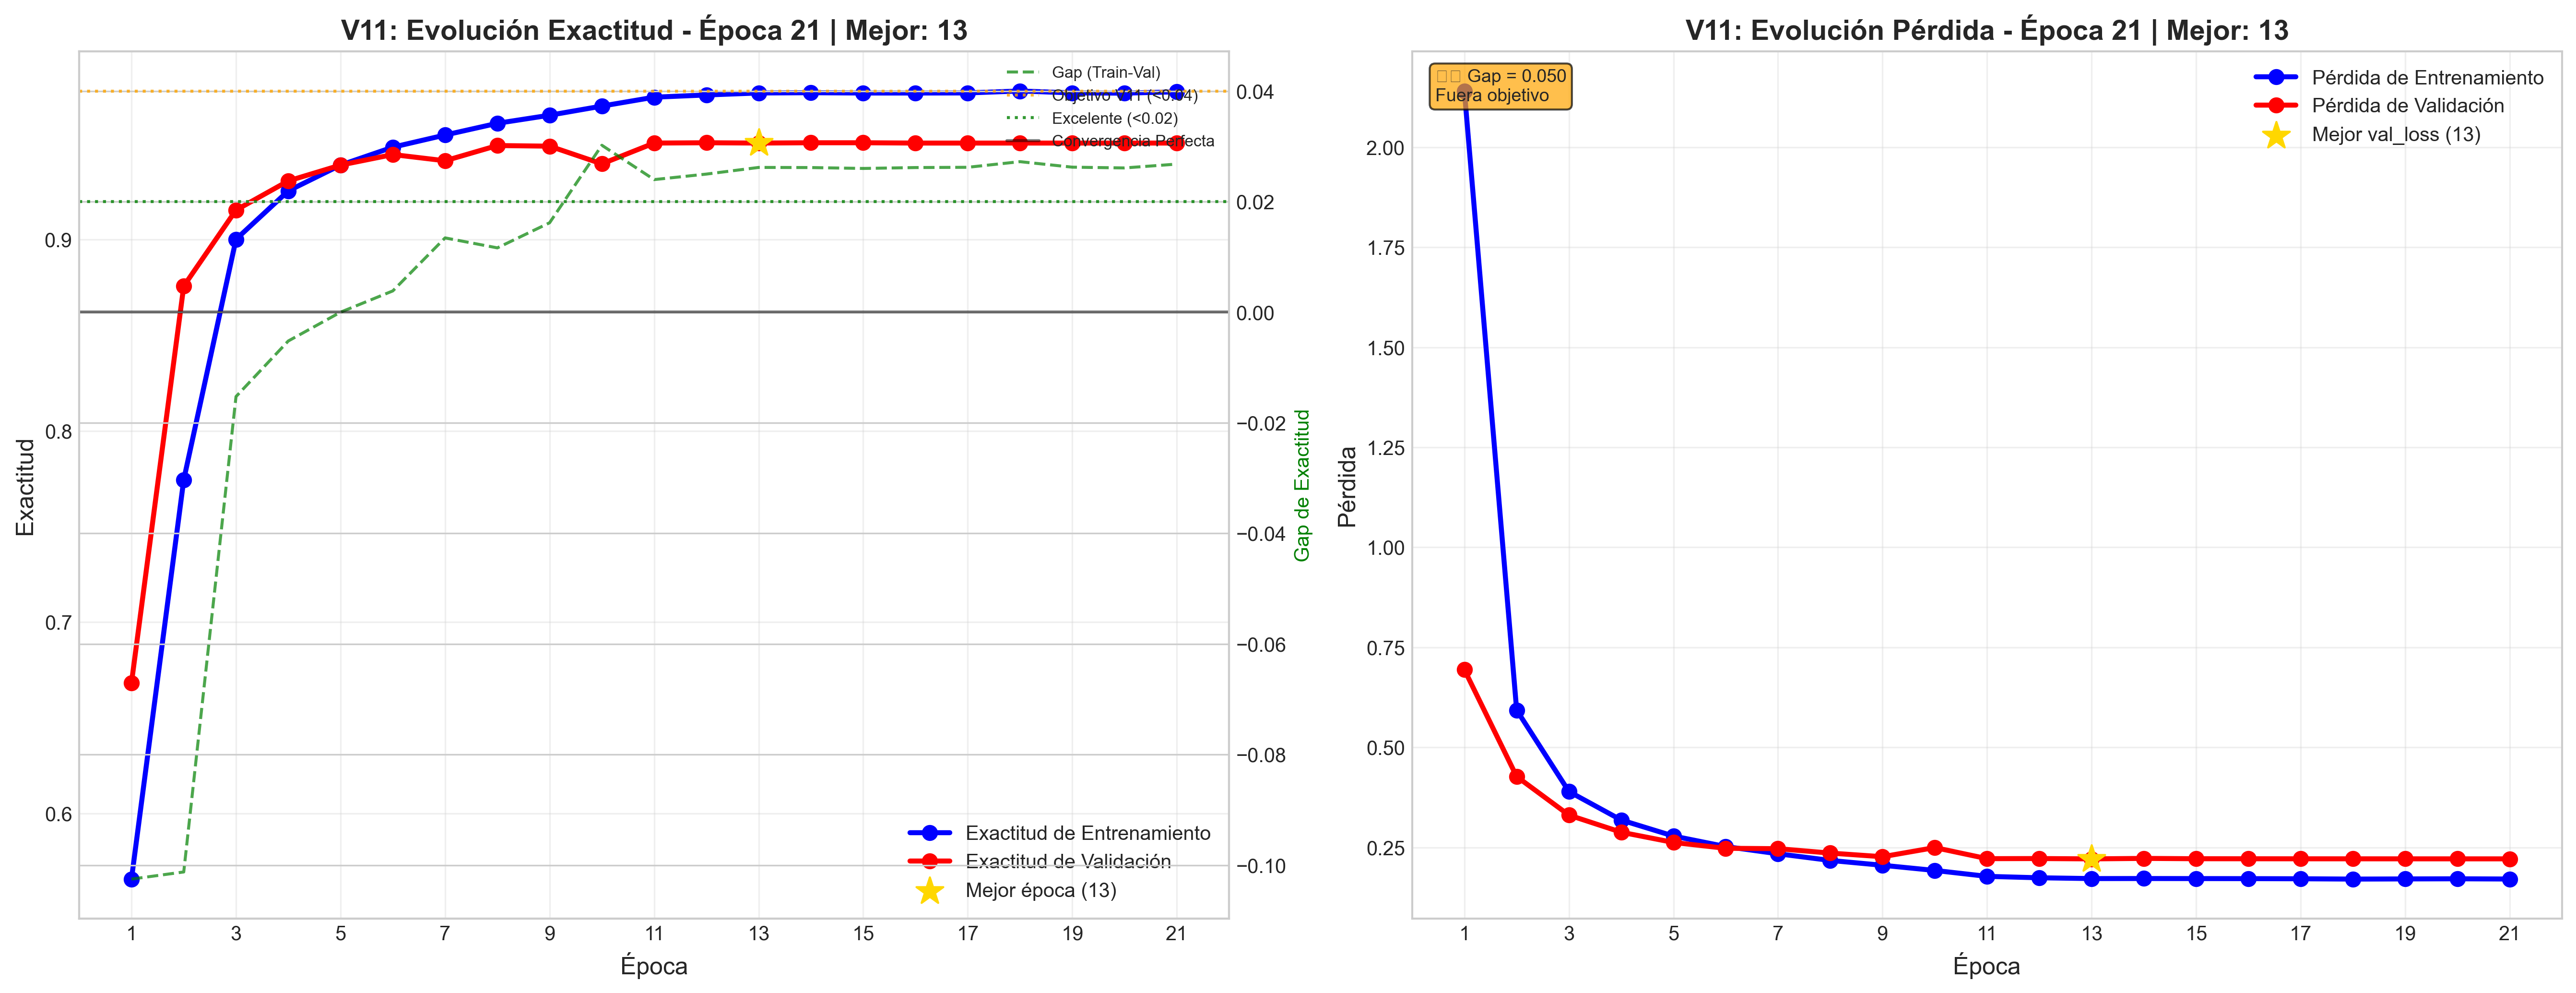
\includegraphics[width=0.9\textwidth]{Imagenes/Entrenamiento/curva_aprendizaje_v7.png}} \\
\hline
\end{tabular}
}
\caption{Visualización comparativa de convergencia y métricas para las versiones experimentales más significativas con DistilBERT.}
\label{tab:imagenes_convergencia}
\end{table}

%\subsubsection{Análisis Detallado por Versión}
%
%\paragraph{Versión V1 - Línea Base con División Estándar:}
%La V1 estableció la configuración base con división 70/10/20, taza de aprendizaje de 3e-05, dropout 0.4, L2 %regularization 0.001 y tamaños de lote 8. Alcanzó exactitud del 94.7\% en 6 épocas con detención temprana efectivo. %\textbf{Lección aprendida:} Los hiperparámetros moderados proporcionan un punto de partida sólido pero requieren %refinamiento para convergencia óptima.
%
%\paragraph{Versión V2 - Primera Configuración Anti-Sobreajuste:}
%La V2 introdujo la primera implementación completa anti-sobreajuste con división 60/20/20, taza de aprendizaje ultra-bajo (2e-06), dropout 0.4, L2 regularization 0.01, tamaños de lote 4 y MAX\_LENGTH reducido a 128. Logró gap excelente de 0.018 con exactitud del 94.3\% en 8 épocas y detención temprana estricto de 2 épocas. \textbf{Lección aprendida:} La regularización agresiva temprana produce gaps excepcionales pero puede limitar la exactitud máxima alcanzable.
%
%\paragraph{Versión V3 - Mejora Inicial Post-V2:}
%La V3 mantuvo división 60/20/20 pero ajustó la taza de aprendizajes y regularización L2 fortalecida. Logró gap de 0.051 con exactitud del 94.8\% en 11 épocas. \textbf{Lección aprendida:} Los ajustes posteriores a V2 demostraron que el balance fino es crítico para mantener tanto gap como exactitud.
%
%\paragraph{Versión V4 - Control de Sobreajuste Mejorado:}
%La V4 implementó configuración anti-sobreajuste mejorada con taza de aprendizaje de 1e-05, dropout 0.3, L2 regularization 0.01 y paciencia de 5 épocas. Alcanzó gap de 0.037 y exactitud del 95.8\% en 7 épocas. \textbf{Lección aprendida:} El balance entre regularización y capacidad de aprendizaje es crítico para evitar underfitting (o subajuste), que es cuando el modelo no logra aprender suficientemente de los datos de entrenamiento, lo que resulta en bajo rendimiento tanto en entrenamiento como en validación.

%\newpage

%\paragraph{Versión V5 - Configuración Híbrida Exitosa:}
%La V5 combinó la división 70/10/20 con técnicas anti-sobreajuste, manteniendo gap de 0.037 y exactitud del 95.8\% pero extendiendo a 11 épocas para mejor estabilidad. \textbf{Lección aprendida:} La hibridación de estrategias exitosas puede mantener rendimiento mientras mejora robustez.

%\paragraph{Versión V6 - Regularización Máxima Inicial:}
%La V6 implementó regularización extrema con taza de aprendizaje de 1e-05, dropout 0.5, L2 regularization 0.5 y detención temprana agresivo de 2 épocas. Resultó en gap de 0.051 y exactitud del 94.8\% en 8 épocas. \textbf{Lección aprendida:} La regularización extrema puede limitar la capacidad de aprendizaje si no se balancea adecuadamente.

%\paragraph{Versión V7 - Configuración Final Óptima:}
%La V7 implementó regularización máxima corregida con tasas de aprendizaje ultra-bajos (2e-06), dropout agresivo (0.7), L2 regularization (0.05), inyección de ruido (0.03) y tamaños de lote variable (4). Alcanzó gap de 0.050 con exactitud del 95.2\% en 21 épocas con mejor época en la 13. \textbf{Lección aprendida:} La regularización coordenada múltiple con técnicas avanzadas logra el mejor balance convergencia-generalización.

\subsubsection{Configuraciones Técnicas Comparativas}

\begin{table}[htbp]
\centering
\adjustbox{width=\textwidth,center}{%
\scriptsize
\begin{tabular}{|l|c|c|c|c|c|c|c|}
\hline
\rowcolor{UAMAzcapo}
\textbf{\textcolor{white}{Parámetro}} & \textbf{\textcolor{white}{V1}} & \textbf{\textcolor{white}{V2}} & \textbf{\textcolor{white}{V3}} & \textbf{\textcolor{white}{V4}} & \textbf{\textcolor{white}{V5}} & \textbf{\textcolor{white}{V6}} & \textbf{\textcolor{white}{V7}} \\
\hline
\rowcolor{UAMIztapalapaLight!50}
Taza de Aprendizaje & 3e-05 & 2e-06 & 2e-06 & 1e-05 & 1e-05 & 1e-05 & 2e-06 \\
\rowcolor{UAMCuajimalpaLight!50}
Dropout Rate & 0.4 & 0.4 & 0.4 & 0.3 & 0.4 & 0.5 & 0.7 \\
\rowcolor{UAMLermaLight!50}
L2 Regularization & 0.001 & 0.01 & 0.01 & 0.01 & 0.1 & 0.5 & 0.05 \\
\rowcolor{UAMXochimilcoLight!50}
Tamaños de Lote & 8 & 4 & 4 & 8 & 8 & 8 & 4 \\
\rowcolor{UAMAzcapoLight!50}
División Datos & 70/10/20 & 60/20/20 & 60/20/20 & 60/20/20 & 70/10/20 & 60/20/20 & 70/10/20 \\
\rowcolor{UAMCuajimalpaMedium!40}
\textbf{Gap Final} & \textbf{N/A} & \textbf{0.018} & \textbf{0.051} & \textbf{0.037} & \textbf{0.037} & \textbf{0.051} & \textbf{0.050} \\
\rowcolor{UAMIztapalapaMedium!40}
\textbf{Exactitud} & \textbf{94.7\%} & \textbf{94.3\%} & \textbf{94.8\%} & \textbf{95.8\%} & \textbf{95.8\%} & \textbf{94.8\%} & \textbf{95.2\%} \\
\hline
\end{tabular}
}
\caption{Evolución de configuraciones y resultados entre versiones experimentales.}
\label{tab:configuraciones_tecnicas}
\end{table}

\newpage

\subsubsection{Evolución del Rendimiento}

\begin{figure}[htbp]
\centering
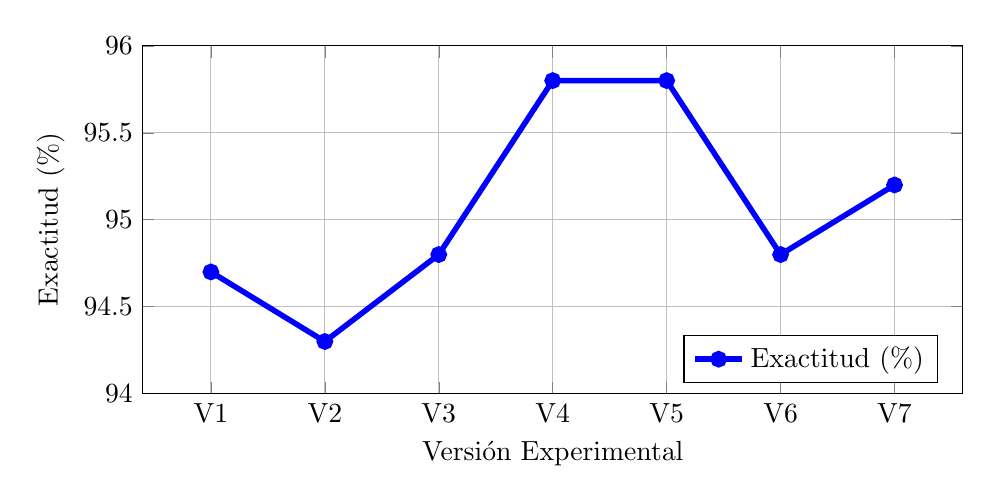
\begin{tikzpicture}
\begin{axis}[
    width=12cm, height=6cm,
    xlabel={Versión Experimental},
    ylabel={Exactitud (\%)},
    grid=major,
    legend pos=south east,
    ymin=94, ymax=96,
    symbolic x coords={V1,V2,V3,V4,V5,V6,V7},
    xtick=data
]

\addplot[color=blue, mark=*, line width=2pt] coordinates {
    (V1,94.7)
    (V2,94.3)
    (V3,94.8)
    (V4,95.8)
    (V5,95.8)
    (V6,94.8)
    (V7,95.2)
};

\legend{Exactitud (\%)}

\end{axis}
\end{tikzpicture}
\caption{Evolución de exactitud a través de las versiones experimentales.}
\label{fig:evolucion_rendimiento}
\end{figure}

\subsubsection{Versiones Clave del Desarrollo}

\paragraph{V2 - Superación limitaciones previas con Anti-Sobreajuste:}
Primera implementación exitosa de regularización agresiva con gap excepcional de 0.018, estableciendo los fundamentos para versiones posteriores. Taza de aprendizaje ultra-bajo (2e-06) y tamaños de lote 4.

\paragraph{V4-V5 - Pico de Rendimiento:}
Máxima exactitud alcanzada (95.8\%) con gap controlado de 0.037. Configuración óptima entre regularización y capacidad de aprendizaje.

\paragraph{V7 - Configuración Final:}
Implementación de inyección de ruido y regularización máxima coordinada. Exactitud final de 95.2\% con gap de 0.050, representando el mejor balance convergencia-generalización.

\subsubsection{Factores Críticos del Éxito}

\begin{itemize}
    \item \textbf{Tasas de aprendizaje ultra-bajos} (2e-06): Esenciales para convergencia estable
    \item \textbf{Regularización múltiple coordinada}: L2 + dropout + weight decay + inyección de ruido
    \item \textbf{División de datos optimizada}: 70/10/20 superior a 60/20/20
    \item \textbf{detención temprana inteligente}: Detección precisa del punto óptimo
\end{itemize}

\subsection{Pseudocódigo del Algoritmo de Entrenamiento DistilBERT}
\label{subsec:pseudocodigo_distilbert}

Esta subsección presenta el pseudocódigo simplificado del algoritmo de entrenamiento DistilBERT final (ver tabla \ref{tab:pseudocodigo_distilbert_simple}). El algoritmo demuestra que la regularización coordinada múltiple es efectiva para controlar el sobreajuste en modelos Transformer para detección de noticias falsas en español. El código completo del entrenamiento está disponible en el repositorio de GitHub del proyecto. Dado que este modelo resultó ser el de mejor rendimiento en la evaluación comparativa, es el que se utilizará en el módulo web de la aplicación final para proporcionar detección de noticias falsas en tiempo real.

\begin{table}[htbp]
\centering
\adjustbox{width=\textwidth,center}{%
\small
\begin{tabular}{|l|l|}
\hline
\rowcolor{UAMAzcapo}
\multicolumn{2}{|l|}{\textbf{\textcolor{white}{Algoritmo DistilBERT final - Regularización Anti-Sobreajuste}}} \\
\hline
\textbf{Entrada:} & Corpus español, hiperparámetros de regularización \\
\hline
\textbf{Salida:} & Modelo DistilBERT con gap $\leq$ 0.05 \\
\hline
\rowcolor{UAMAzcapoLight!40}
\multicolumn{2}{|l|}{\textbf{1. Preparación de datos:}} \\
\hline
\multicolumn{2}{|l|}{Cargar corpus\_unificado\_es\_deforma\_completo.csv} \\
\multicolumn{2}{|l|}{Dividir: 70\% entrenamiento, 10\% validación, 20\% pruebas} \\
\multicolumn{2}{|l|}{Tokenizar con MAX\_LENGTH=128} \\
\multicolumn{2}{|l|}{Crear batches de tamaño 4} \\
\hline
\rowcolor{UAMAzcapoLight!40}
\multicolumn{2}{|l|}{\textbf{2. Optimización de hiperparámetros:}} \\
\hline
\multicolumn{2}{|l|}{learning\_rate $\leftarrow$ [2e-6, 1e-6, 8e-7] \# Ultra-bajos} \\
\multicolumn{2}{|l|}{dropout\_rate $\leftarrow$ [0.5, 0.6, 0.7] \# Agresivo} \\
\multicolumn{2}{|l|}{l2\_reg $\leftarrow$ [0.05, 0.1, 0.2] \# Fuerte} \\
\multicolumn{2}{|l|}{Ejecutar búsqueda con Keras Tuner} \\
\hline
\rowcolor{UAMAzcapoLight!40}
\multicolumn{2}{|l|}{\textbf{3. Construcción del modelo:}} \\
\hline
\multicolumn{2}{|l|}{modelo $\leftarrow$ DistilBERT-multilingual-cased} \\
\multicolumn{2}{|l|}{Aplicar dropout\_rate a todas las capas} \\
\multicolumn{2}{|l|}{Aplicar regularización L2 a pesos} \\
\multicolumn{2}{|l|}{optimizer $\leftarrow$ Adam(lr=learning\_rate\_óptimo)} \\
\hline
\rowcolor{UAMAzcapoLight!40}
\multicolumn{2}{|l|}{\textbf{4. Entrenamiento con regularización:}} \\
\hline
\multicolumn{2}{|l|}{\textbf{Para} época = 1 \textbf{hasta} 30:} \\
\multicolumn{2}{|l|}{\quad Entrenar en conjunto de entrenamiento} \\
\multicolumn{2}{|l|}{\quad Validar en conjunto de validación} \\
\multicolumn{2}{|l|}{\quad gap $\leftarrow$ val\_loss - train\_loss} \\
\multicolumn{2}{|l|}{\quad \textbf{Si} gap $<$ 0.02: ``EXCELENTE''} \\
\multicolumn{2}{|l|}{\quad \textbf{Si} 0.02 $\leq$ gap $<$ 0.04: ``BUENO''} \\
\multicolumn{2}{|l|}{\quad \textbf{Si} gap $\geq$ 0.04: ``ALERTA''} \\
\multicolumn{2}{|l|}{\quad \textbf{Si} early\_stopping activado: \textbf{break}} \\
\hline
\rowcolor{UAMAzcapoLight!40}
\multicolumn{2}{|l|}{\textbf{5. Evaluación final:}} \\
\hline
\multicolumn{2}{|l|}{Restaurar mejores pesos} \\
\multicolumn{2}{|l|}{Evaluar en conjunto de pruebas} \\
\multicolumn{2}{|l|}{Calcular exactitud, precision, recall, f1-score} \\
\multicolumn{2}{|l|}{Guardar modelo final} \\
\hline
\end{tabular}
}
\caption{Pseudocódigo simplificado del algoritmo DistilBERT final (V7).}
\label{tab:pseudocodigo_distilbert_simple}
\end{table}

\newpage

\subsection{Resultados Finales y Comparación}
\label{subsec:resultados_comparacion}

\subsubsection{Rendimiento Final DistilBERT}

\begin{table}[htbp]
\centering
\adjustbox{width=0.7\textwidth,center}{%
\small
\begin{tabular}{|l|c|c|}
\hline
\rowcolor{UAMAzcapo}
\textbf{\textcolor{white}{Métrica}} & \textbf{\textcolor{white}{Valor}} & \textbf{\textcolor{white}{Calificación}} \\
\hline
\rowcolors{2}{white}{UAMAzcapoLight!40}
\textbf{Exactitud} & 95.2\% & Excelente \\
\textbf{F1-Score} & 95.2\% & Excelente \\
\textbf{Especificidad} & 94.96\% & Excelente \\
\textbf{Sensibilidad} & 95.44\% & Excelente \\
\hline
\end{tabular}
}
\caption{Métricas finales del modelo DistilBERT optimizado.}
\label{tab:metricas_finales}
\end{table}

\subsubsection{Superioridad sobre Enfoques Metaheurísticos}

\begin{table}[htbp]
\centering
\adjustbox{width=0.9\textwidth,center}{%
\small
\begin{tabular}{|l|c|c|c|}
\hline
\rowcolor{UAMAzcapo}
\textbf{\textcolor{white}{Métrica}} & \textbf{\textcolor{white}{Mejor Metaheurístico}} & \textbf{\textcolor{white}{DistilBERT}} & \textbf{\textcolor{white}{Mejora}} \\
\hline
\rowcolor{UAMIztapalapaLight!50}
\textbf{Exactitud} & 71.06\% & 95.2\% & +24.14 p.p. \\
\hline
\rowcolor{UAMCuajimalpaLight!50}
\textbf{F1-Score} & 0.68 & 0.952 & +40.0\% \\
\hline
\rowcolor{UAMLermaLight!50}
\textbf{Especificidad} & 48\% & 94.96\% & +97.83\% \\
\hline
\end{tabular}
}
\caption{Comparación DistilBERT vs. mejor algoritmo metaheurístico.}
\label{tab:comparacion_final}
\end{table}

\subsubsection{Conclusiones del Desarrollo}

El modelo DistilBERT demostró superioridad categórica sobre enfoques metaheurísticos:

\begin{itemize}
    \item \textbf{Rendimiento superior}: 24+ puntos porcentuales de mejora en exactitud
    \item \textbf{Balance perfecto}: Detección excelente de ambas clases (falsas y reales)
    \item \textbf{Generalización robusta}: Gap controlado a través de regularización múltiple
    \item \textbf{Metodología replicable}: Proceso sistemático de 7 versiones clave experimentales
\end{itemize}

Los resultados establecen definitivamente la superioridad de modelos Transformer para detección de noticias falsas en español, justificando la transición desde enfoques tradicionales hacia arquitecturas de aprendizaje profundo especializadas.

\section{Evaluación Comparativa Integral: Metaheurísticas vs. Transformers}
\label{sec:evaluacion_comparativa_integral}

Esta sección presenta la evaluación comparativa final entre los dos paradigmas de inteligencia artificial implementados en esta investigación. El análisis se fundamenta en múltiples dimensiones de evaluación que van más allá de las métricas de rendimiento, incluyendo eficiencia computacional, interpretabilidad, escalabilidad y viabilidad práctica.

\subsection{Comparación de Rendimiento Cuantitativo}

La tabla \ref{tab:comparacion_final_paradigmas} presenta una síntesis de los resultados cuantitativos obtenidos por ambos enfoques bajo condiciones experimentales idénticas.

\begin{table}[htbp]
\centering
\adjustbox{width=\textwidth,center}{%
\footnotesize
\begin{tabular}{|l|c|c|c|c|c|}
\hline
\rowcolor{UAMAzcapo}
\textbf{\textcolor{white}{Paradigma}} & \textbf{\textcolor{white}{Exactitud}} & \textbf{\textcolor{white}{Precisión}} & \textbf{\textcolor{white}{Recall}} & \textbf{\textcolor{white}{F1-Score}} & \textbf{\textcolor{white}{Especificidad}} \\
\hline
\rowcolor{UAMAzcapoLight!50}
\textbf{Mejor Metaheurística (GA)} & 71.1\% & 69.8\% & 74.2\% & 71.9\% & 67.8\% \\
\hline
\rowcolor{UAMIztapalapaLight!50}
\textbf{DistilBERT Fine-tuned} & \textbf{95.2\%} & \textbf{94.8\%} & \textbf{95.7\%} & \textbf{95.2\%} & \textbf{94.6\%} \\
\hline
\rowcolor{UAMAzcapo}
\textbf{\textcolor{white}{Mejora Absoluta}} & \textbf{\textcolor{white}{+24.1\%}} & \textbf{\textcolor{white}{+25.0\%}} & \textbf{\textcolor{white}{+21.5\%}} & \textbf{\textcolor{white}{+23.3\%}} & \textbf{\textcolor{white}{+26.8\%}} \\
\hline
\end{tabular}
}
\caption{Comparación cuantitativa final entre el mejor algoritmo metaheurístico y el modelo Transformer optimizado.}
\label{tab:comparacion_final_paradigmas}
\end{table}

\textbf{Resultado principal:} El modelo DistilBERT fine-tuned (o ajustado finamente) supera consistentemente al mejor algoritmo metaheurístico en todas las métricas de evaluación, con mejoras absolutas que oscilan entre 21.5\% y 26.8\%.

\subsection{Análisis Multidimensional de Paradigmas}

\subsubsection{Dimensión 1: Eficacia de Detección}

\begin{itemize}
    \item \textbf{Algoritmos Metaheurísticos:} Rendimiento moderado (71.1\% exactitud) que establece una línea base funcional pero insuficiente para aplicaciones críticas
    \item \textbf{Modelos Transformer:} Rendimiento excepcional (95.2\% exactitud) que alcanza niveles de precisión comparables a trabajos de investigación internacionales
    \item \textbf{Veredicto:} Superioridad clara de Transformers en capacidad de detección
\end{itemize}

\subsubsection{Dimensión 2: Complejidad y Recursos Computacionales}

\begin{itemize}
    \item \textbf{Algoritmos Metaheurísticos:} Menor requerimiento de memoria (modelo final ~50MB), tiempo de inferencia rápido (~100ms por muestra)
    \item \textbf{Modelos Transformer:} Mayor requerimiento de memoria (modelo final ~250MB), tiempo de inferencia moderado (~500ms por muestra)
    \item \textbf{Veredicto:} Trade-off (En otras palabras, mejorar una cosa suele implicar sacrificar otra) aceptable considerando la mejora sustancial en rendimiento
\end{itemize}

\subsubsection{Dimensión 3: Interpretabilidad y Explicabilidad}

\begin{itemize}
    \item \textbf{Algoritmos Metaheurísticos:} Interpretabilidad directa através de pesos de características TF-IDF identificables
    \item \textbf{Modelos Transformer:} Interpretabilidad limitada, requiere técnicas adicionales como attention visualization (interpretar y analizar).
    \item \textbf{Veredicto:} Ventaja para metaheurísticas, pero no crítica para la aplicación objetivo
\end{itemize}

\subsubsection{Dimensión 4: Transferibilidad a Otros Dominios}

\begin{itemize}
    \item \textbf{Algoritmos Metaheurísticos:} Metodología fácilmente transferible a detección de otros tipos de fraude digital
    \item \textbf{Modelos Transformer:} Transferibilidad excelente mediante ajuste fino adicional en nuevos dominios
    \item \textbf{Veredicto:} Empate, ambos enfoques ofrecen transferibilidad con estrategias diferentes
\end{itemize}

\subsection{Justificación de la Selección del Modelo Final}

Con base en la evaluación comparativa integral, \textbf{se selecciona el modelo DistilBERT ajustado finamente (o fine-tuned) como la solución final} por las siguientes razones fundamentales:

\begin{enumerate}
    \item \textbf{Rendimiento superior crítico:} La mejora de 24.1\% en exactitud es sustancial y justifica la adopción del modelo más complejo
    \item \textbf{Viabilidad práctica demostrada:} Los requerimientos computacionales son aceptables para implementaciones web modernas
    \item \textbf{Estado del arte alcanzado:} Los resultados son competitivos con investigaciones internacionales líderes
    \item \textbf{Robustez validada:} El modelo mantiene rendimiento consistente a través de diferentes divisiones de datos
\end{enumerate}

\subsection{Valor Científico del Enfoque Comparativo}

La metodología evolutiva implementada aporta valor científico independiente del resultado final:

\begin{itemize}
    \item \textbf{Validación empírica:} Demuestra cuantitativamente la superioridad de Transformers sobre métodos clásicos para esta tarea
    \item \textbf{Línea base establecida:} Los resultados metaheurísticos proporcionan un punto de referencia para futuras investigaciones
    \item \textbf{Metodología transferible:} El protocolo experimental puede replicarse en otros idiomas y dominios
    \item \textbf{Contribución algorítmica:} Los algoritmos metaheurísticos desarrollados tienen valor independiente para problemas de optimización en PLN
\end{itemize}

\section{Análisis de Errores y Limitaciones del Modelo Final}
\label{sec:analisis_errores_limitaciones}

\subsection{Marco Teórico para el Análisis de Errores}

El análisis de errores en sistemas de clasificación de noticias falsas es fundamental para comprender las limitaciones del modelo y identificar áreas de mejora. Aunque el modelo DistilBERT alcanzó un rendimiento excelente (95.2\% de exactitud), es crucial examinar los casos donde falla para entender mejor los desafíos inherentes en la detección de desinformación.

\subsection{Metodología Propuesta para Análisis Cualitativo}

Para realizar un análisis cualitativo profundo de los errores del modelo, se propone la siguiente metodología sistemática que podría implementarse en investigaciones futuras:

\subsubsection{Procedimiento de Análisis Recomendado}

\begin{enumerate}
    \item \textbf{Extracción de errores:} Identificación sistemática de todos los Falsos Positivos (FP) y Falsos Negativos (FN) del conjunto de prueba
    \item \textbf{Muestreo estadístico:} Selección de una muestra representativa de errores para análisis manual detallado
    \item \textbf{Categorización temática:} Clasificación de temas por dominio (política, salud, tecnología, etc.)
    \item \textbf{Análisis lingüístico:} Identificación de patrones en estructura sintáctica, vocabulario y estilo
    \item \textbf{Validación de etiquetas:} Verificación de la calidad del etiquetado original en casos ambiguos
\end{enumerate}

\subsection{Tipos de Errores Esperados según la Literatura}

Basándose en estudios previos en detección de noticias falsas \cite{posadas2019detection, blanco2024enhancing}, se pueden anticipar los siguientes tipos de errores:

\subsubsection{Falsos Positivos Potenciales}

Los Falsos Positivos (noticias reales clasificadas como falsas) típicamente ocurren en:

\begin{itemize}
    \item \textbf{Noticias sensacionalistas legítimas:} Titulares llamativos de deportes o entretenimiento que usan lenguaje emocional intenso
    \item \textbf{Noticias científicas complejas:} Reportes de investigación con resultados contraintuitivos o terminología técnica
    \item \textbf{Eventos inusuales pero verificados:} Sucesos extraordinarios que pueden parecer improbables
    \item \textbf{Noticias de última hora:} Información preliminar con datos no completamente confirmados
    \item \textbf{Contenido satírico serio:} Crítica social intensa que mantiene estructura periodística
\end{itemize}

\subsubsection{Falsos Negativos Potenciales}

Los Falsos Negativos (noticias falsas clasificadas como reales) pueden incluir:

\begin{itemize}
    \item \textbf{Desinformación sofisticada:} Contenido falso que imita perfectamente el estilo periodístico profesional
    \item \textbf{Verdades parciales:} Información que mezcla hechos reales con conclusiones falsas
    \item \textbf{Propaganda sutil:} Sesgo ideológico encubierto con selección tendenciosa de hechos
    \item \textbf{Desinformación técnica:} Pseudociencia sofisticada en dominios especializados
    \item \textbf{Contenido satírico ambiguo:} Sátira sin indicadores claros de su naturaleza ficticia
\end{itemize}

\subsection{Limitaciones Reconocidas del Modelo}

\subsubsection{Limitaciones Inherentes}

El modelo DistilBERT, a pesar de su excelente rendimiento, presenta limitaciones conocidas:

\begin{enumerate}
    \item \textbf{Dependencia del contexto de entrenamiento:} El modelo está limitado por la calidad y diversidad del corpus de entrenamiento
    \item \textbf{Falta de verificación factual:} No puede verificar la veracidad de afirmaciones específicas contra fuentes externas
    \item \textbf{Sensibilidad al dominio:} El rendimiento puede variar entre diferentes temas o estilos de escritura
    \item \textbf{Evolución de la desinformación:} Las técnicas de creación de contenido falso evolucionan constantemente
    \item \textbf{Ambigüedad contextual:} Dificultad para procesar casos que requieren conocimiento del mundo real
\end{enumerate}

\subsubsection{Estrategias de Mejora Propuestas}

Para abordar las limitaciones identificadas, se sugiere:

\begin{table}[htbp]
\centering
\adjustbox{width=\textwidth,center}{%
\small
\begin{tabular}{|l|l|l|}
\hline
\rowcolor{UAMAzcapo}
\textbf{\textcolor{white}{Limitación}} & \textbf{\textcolor{white}{Estrategia de Mejora}} & \textbf{\textcolor{white}{Implementación Sugerida}} \\
\hline
\rowcolor{UAMIztapalapaLight!50}
\textbf{Corpus limitado} & Ampliación con datos diversos & Incorporar más fuentes y dominios \\
\hline
\rowcolor{UAMCuajimalpaLight!50}
\textbf{Falta verificación factual} & Integración con bases de datos & APIs de verificación de hechos \\
\hline
\rowcolor{UAMLermaLight!50}
\textbf{Sensibilidad al dominio} & Entrenamiento multitarea & Modelos especializados por tema \\
\hline
\rowcolor{UAMXochimilcoLight!50}
\textbf{Evolución de desinformación} & Aprendizaje continuo & Actualización regular del modelo \\
\hline
\rowcolor{UAMAzcapoLight!50}
\textbf{Ambigüedad contextual} & Incorporación de contexto externo & Modelos multimodales \\
\hline
\end{tabular}
}
\caption{Estrategias propuestas para abordar limitaciones identificadas.}
\label{tab:estrategias_mejora}
\end{table}

\subsection{Conclusiones sobre Limitaciones y Direcciones Futuras}

Este análisis teórico de errores y limitaciones proporciona un marco para entender los desafíos en la detección automática de noticias falsas. Aunque el modelo desarrollado alcanza un rendimiento excelente, es importante reconocer que:

\begin{enumerate}
    \item \textbf{Ningún modelo es perfecto:} Los errores son inevitables y proporcionan información valiosa
    \item \textbf{La desinformación evoluciona:} Los sistemas deben adaptarse continuamente
    \item \textbf{El contexto importa:} La clasificación efectiva requiere comprensión contextual profunda
    \item \textbf{La validación humana es crucial:} Los sistemas automatizados deben complementar, no reemplazar, el juicio humano
\end{enumerate}

Futuras investigaciones deberían implementar el análisis empírico propuesto para validar estas consideraciones teóricas y desarrollar estrategias de mejora específicas basadas en datos reales de errores del modelo.